% !TEX root = main.tex

% TODO:
% REMARK:

\section{Asymmetry Bias}
\label{sec:AsymBias}

	In the standard model(SM), the $A_{cp}$ of $t\bar{t}$ and other background are expected to be zero, that is to say, there is no asymmetry. However, the $A'_{cp}$ value may be affected by the reconstructing and detector demonstrating, and also the particles' characteristic may interact with detector, so the $A'_{cp}$ might be different from the real $A_{cp}$. And the reconstruction effects from the detector can be studied by simulation sample. Also, the detector and reconstruction bias is expected to be the major systematic uncertainty of the analysis.

	The best way to estimate the detector and reconstruction issue is to see the $A'_{cp}$ bias of a sample which supposes to be zero in $A_{cp}$. And then, the standard deviation(error) of $A'_{cp}$ is taken as the detector and reconstruction bias. The sample needs to be irrelavent with the target signal of this analysis -- $t\bar{t}$ because we expect the possible source of asymmetry is in $t\bar{t}$. Accordingly, the SR background sample is appropriate to be studied for the detector and reconstruction bias since it is supposed to be without $A_{cp}$ and it is nothing relative to the signal in the analysis($t\bar{t}$). However, the SR background sample has low statistics. Therefore, the method in 8TeV analysis is using the W+jets-dominant CR data sample as the sample supposed to be without $A_{cp}$, because the W+jets CR data sample is used to data-driven the SR background sample. Yet, in this analysis, we use the analyzed data itself and a fake data method to doing this study. It is advatage of using SR data itself that the statistics is more than CR data and that the W+jets-dominant CR smaple still includes over $10\%$ $t\bar{t}$. And the chapter is to introduce the fake data method to calculate the detector and reconstruction bias.

	\subsection{Asymmetry in simulation sample}
	\label{ssec:Asym_in_sim}

		There are the $A'_{cp}$ of simulated $t\bar{t}$ sample in SR with 3 different reconstruction results($\chi^2_{min}$, MVA-A, MVA-B). It is expected to have no asymmetry because of the simulation sample is generated based on standard model(SM).


		\begin{figure}[H]
			\centering
				\subfigure[Muon channel]{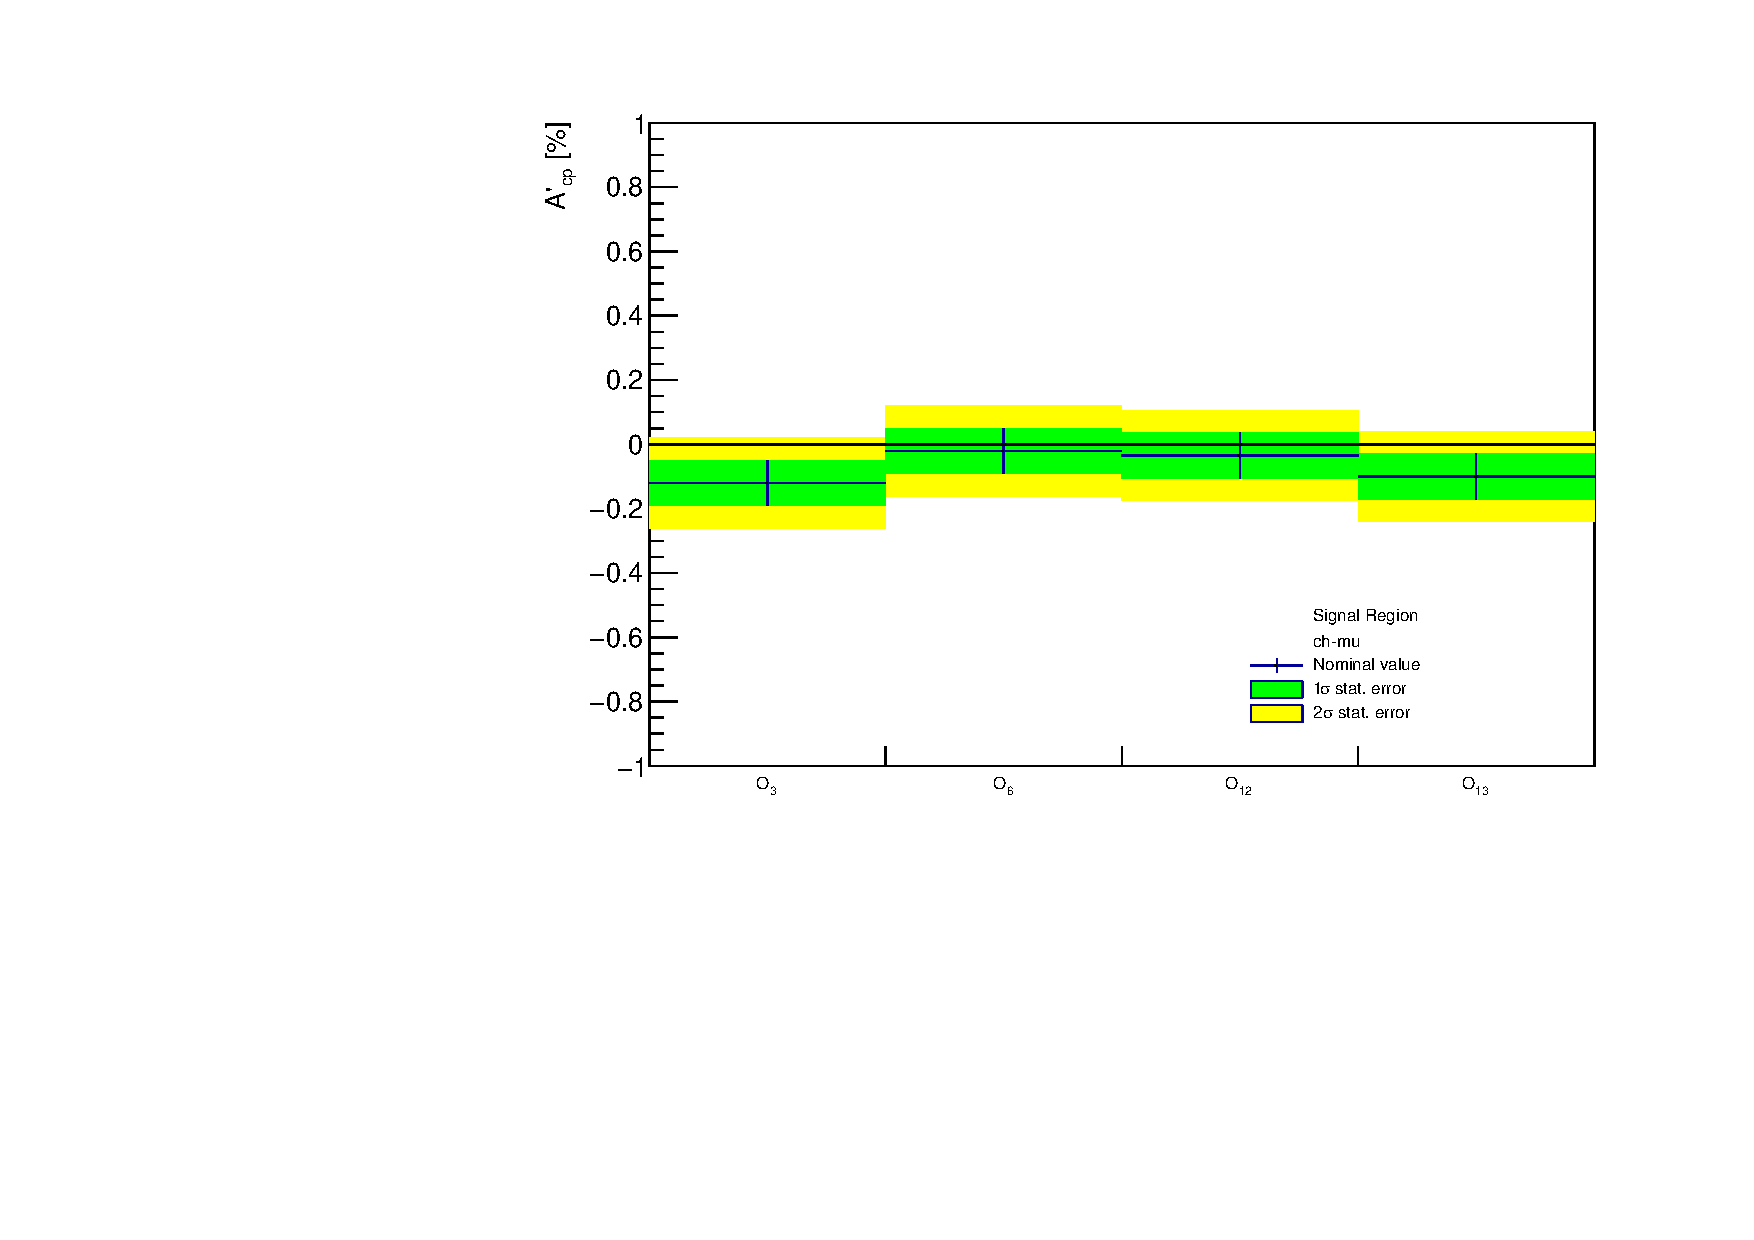
\includegraphics[width=0.45\textwidth]{Figures/Asym/check/Acp_chi2_Mlbcut_DetBiasAcp_SRtt_200928_2217_mu.pdf}}
				\subfigure[Electron channel]{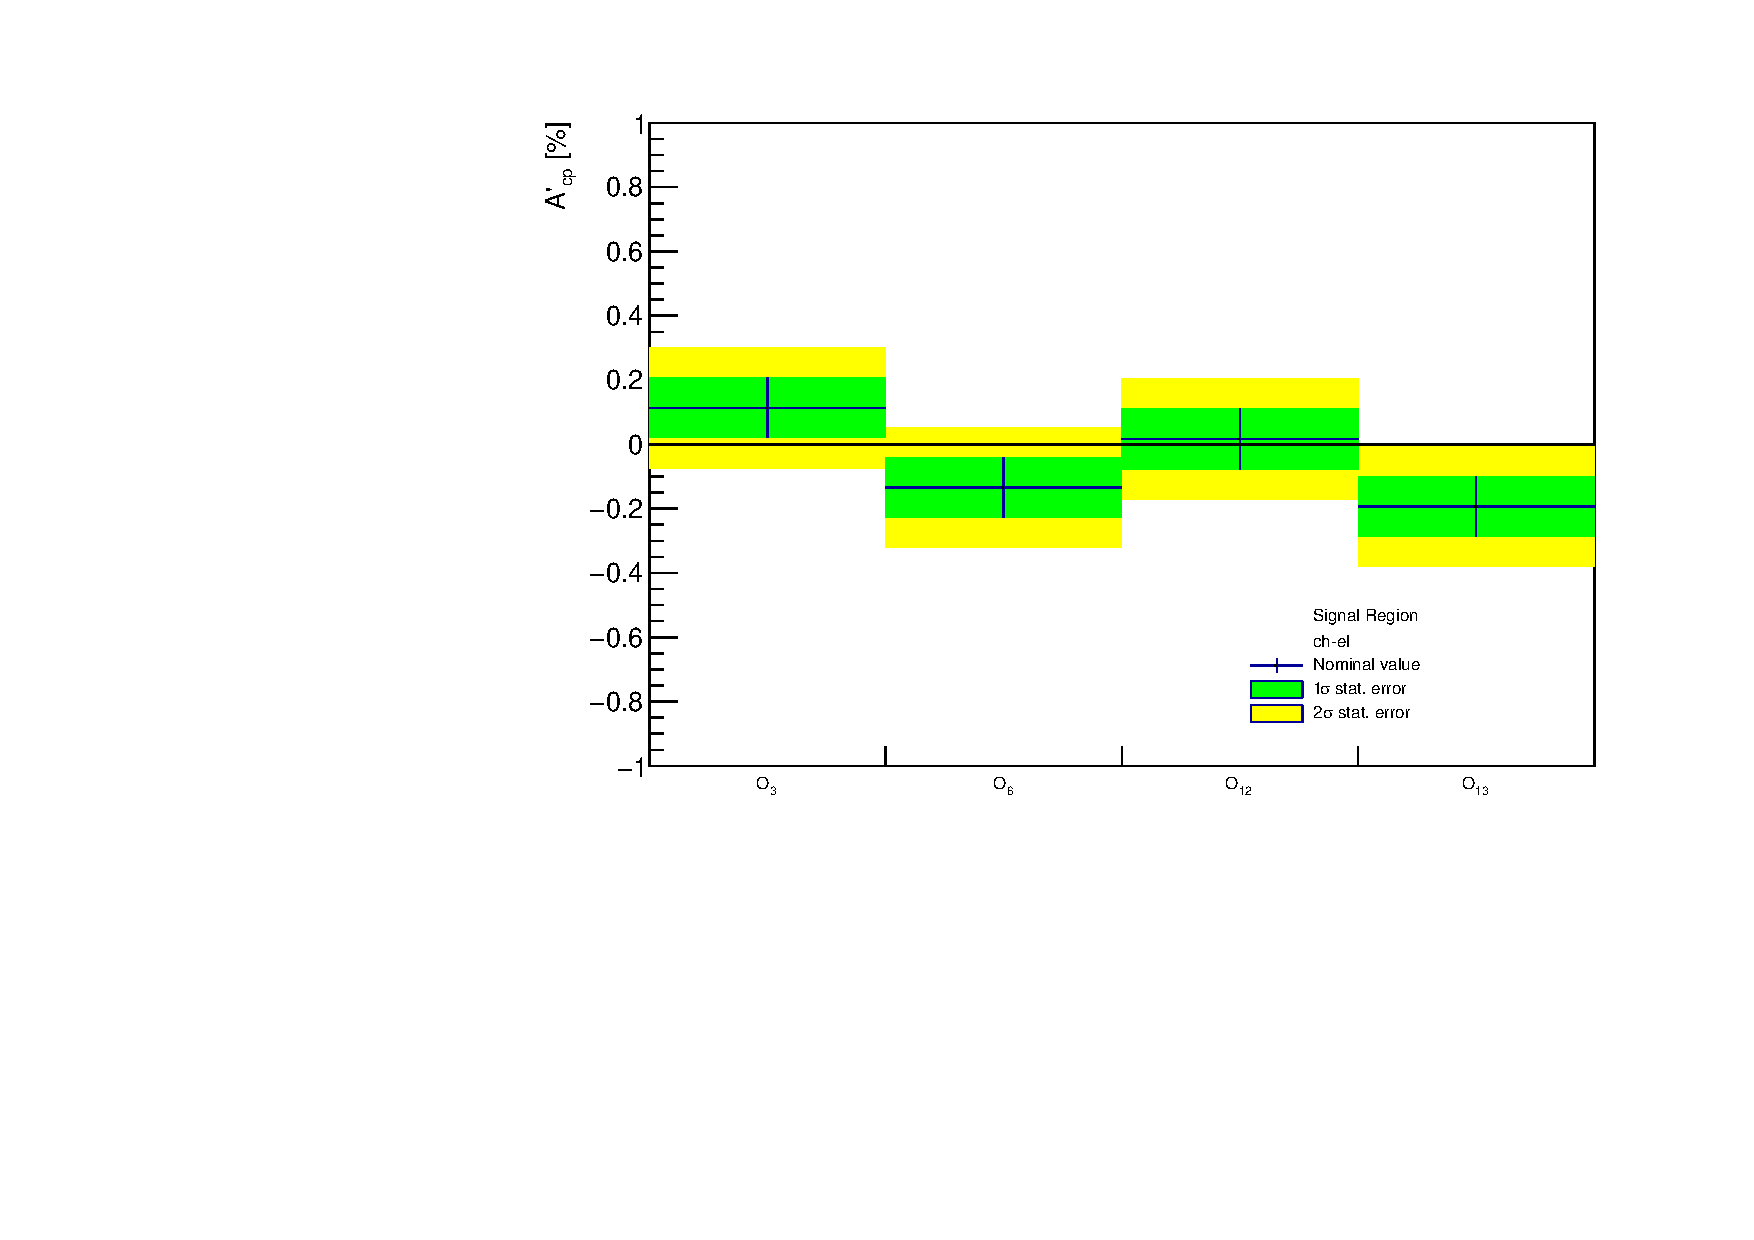
\includegraphics[width=0.45\textwidth]{Figures/Asym/check/Acp_chi2_Mlbcut_DetBiasAcp_SRtt_200928_2217_el.pdf}}\\
		\caption{$A'_{cp}$ of simulated signal sample($t\bar{t}$) by $\chi^2_{min}$ reconstruction strategy}
		\label{AsymBias:fig:chi2_sim_tt_A'cp}
		\end{figure}
		\FloatBarrier

		\begin{figure}[H]
			\centering
				\subfigure[Muon channel]{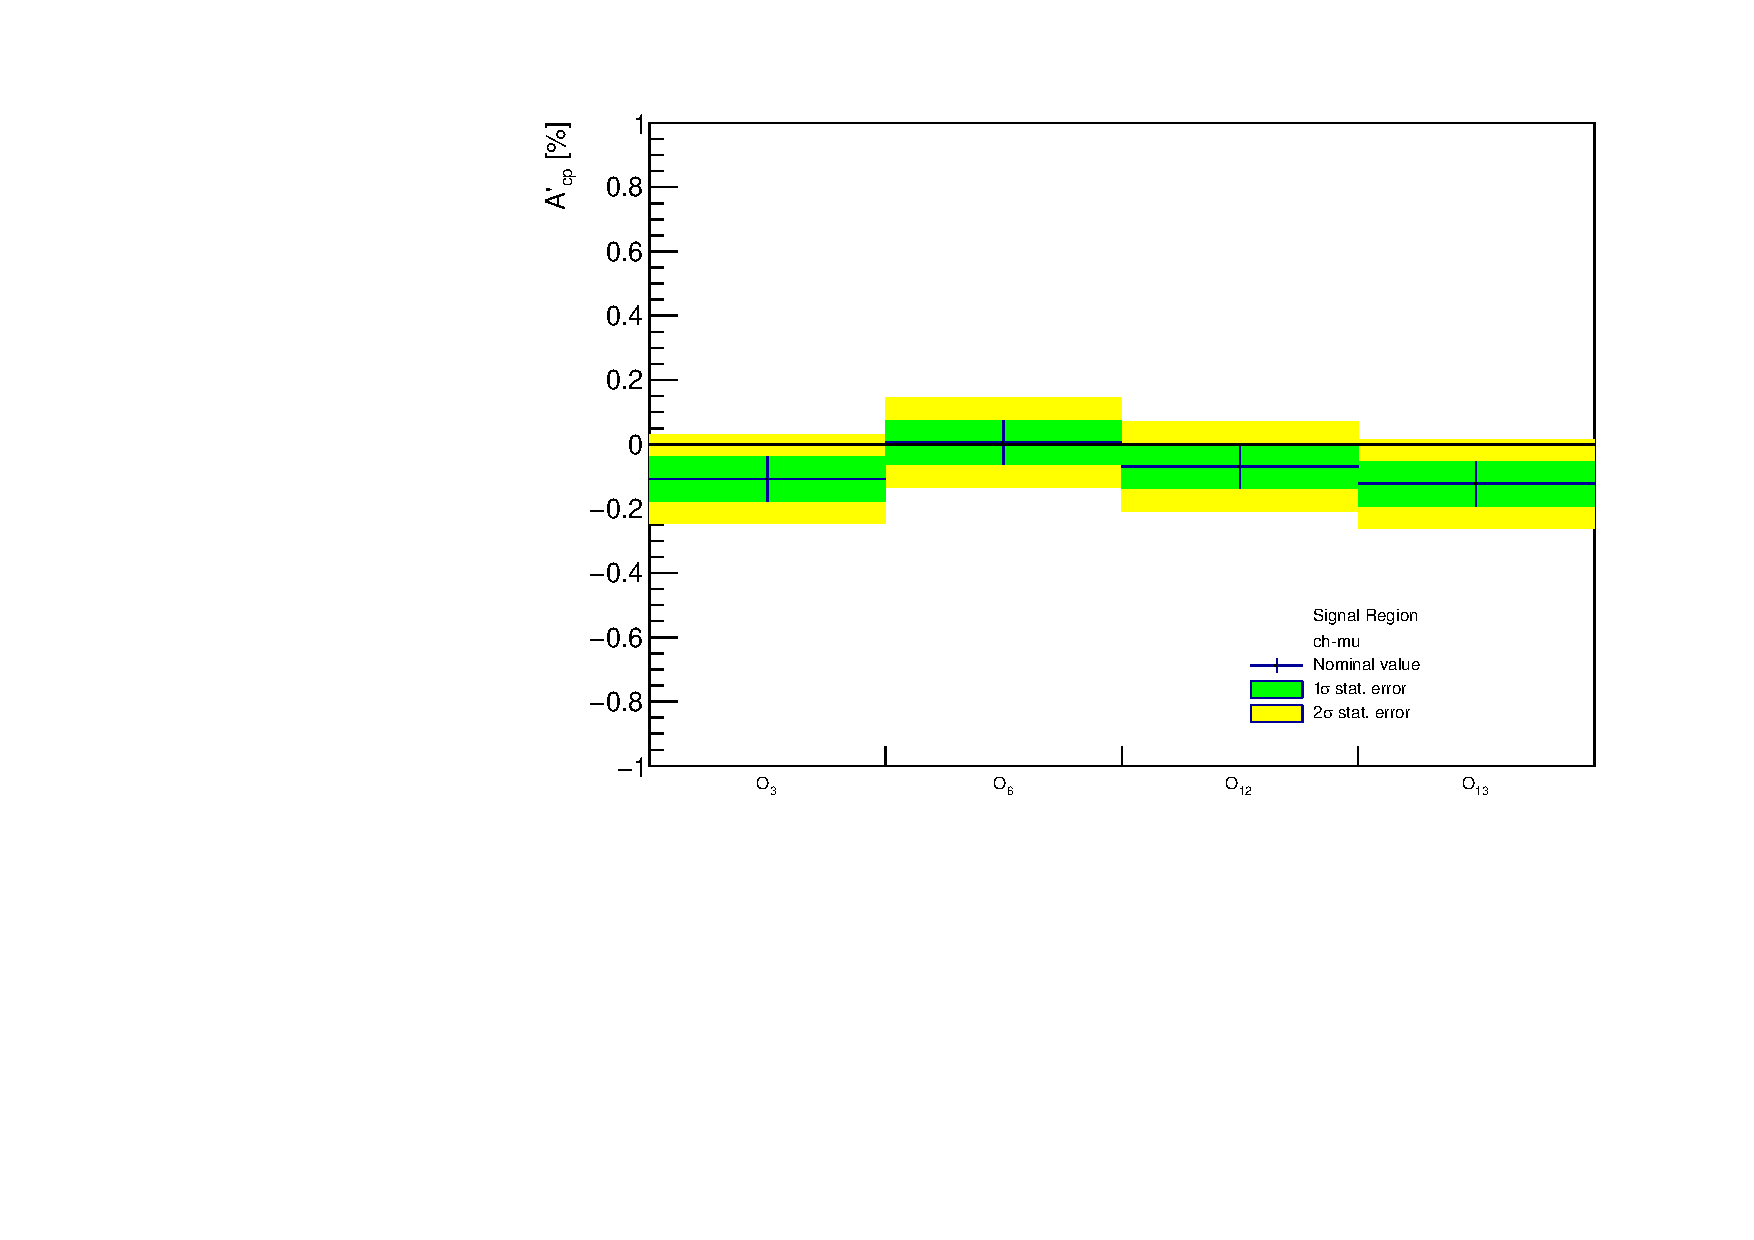
\includegraphics[width=0.45\textwidth]{Figures/Asym/check/Acp_a05_MLP_Mlbcut_DetBiasAcp_SRtt_200928_2222_mu.pdf}}
				\subfigure[Electron channel]{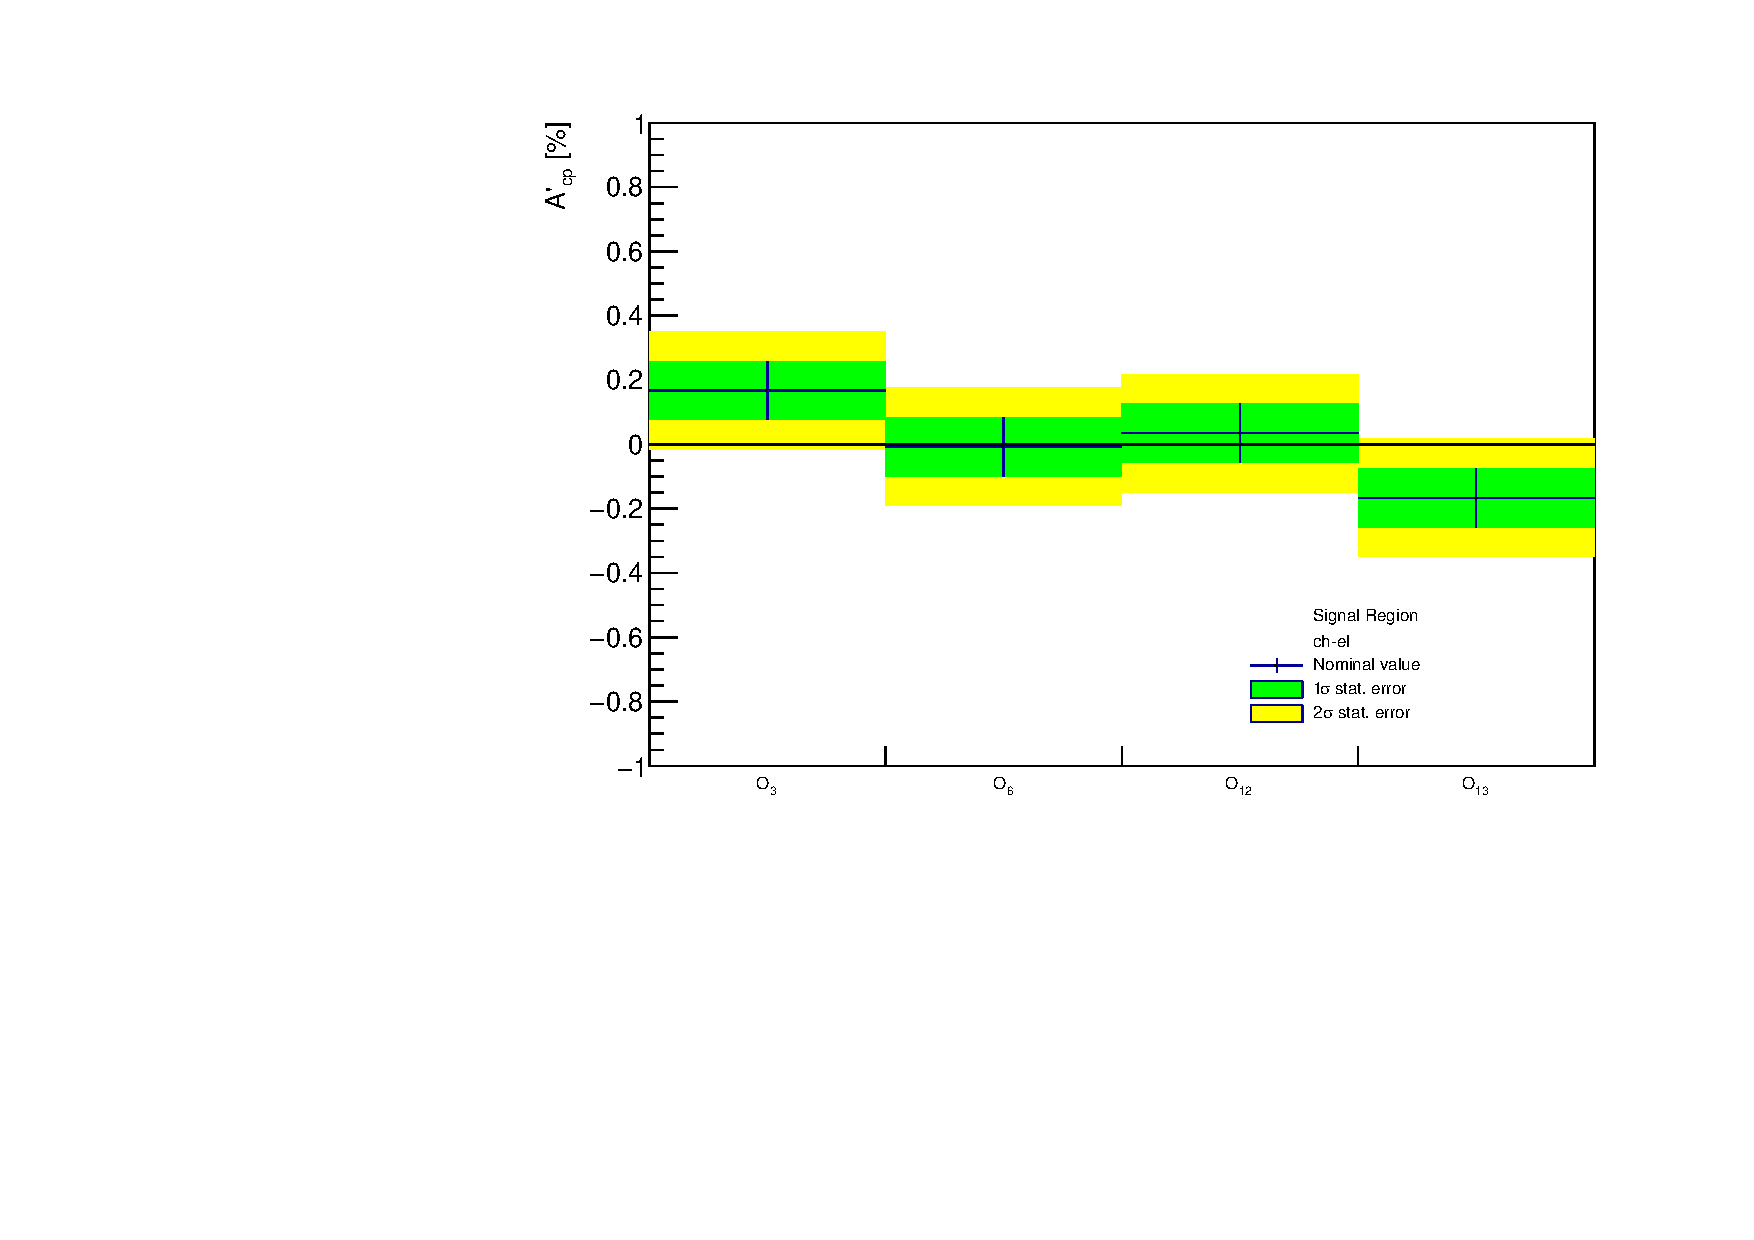
\includegraphics[width=0.45\textwidth]{Figures/Asym/check/Acp_a05_MLP_Mlbcut_DetBiasAcp_SRtt_200928_2222_el.pdf}}\\
		\caption{$A'_{cp}$ of simulated signal sample($t\bar{t}$) by MVA-A reconstruction strategy}
		\label{AsymBias:fig:a05_Mlbcut_sim_tt_A'cp}
		\end{figure}
		\FloatBarrier

		\begin{figure}[H]
			\centering
				\subfigure[Muon channel]{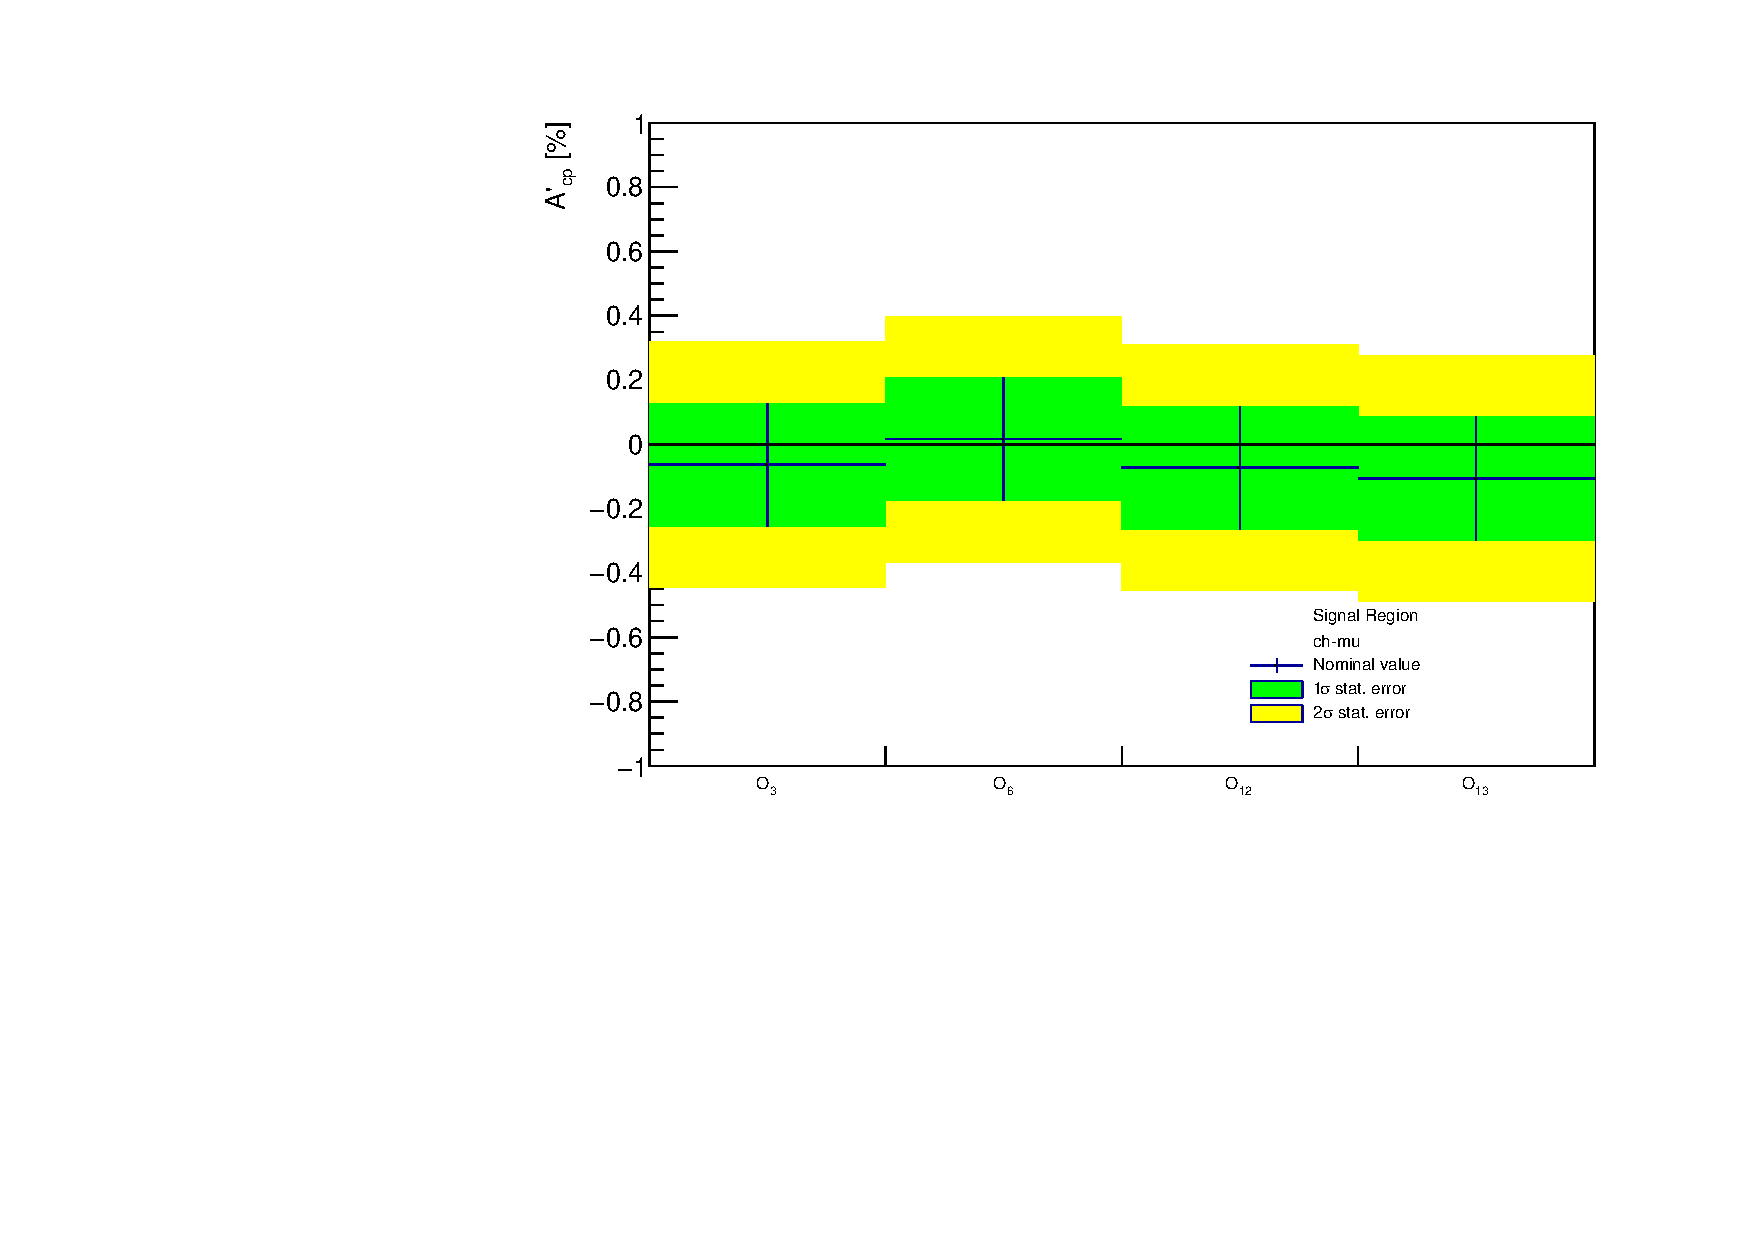
\includegraphics[width=0.45\textwidth]{Figures/Asym/check/Acp_a05_MLP_noMlbcut_DetBiasAcp_SRtt_200928_2219_mu.pdf}}
				\subfigure[Electron channel]{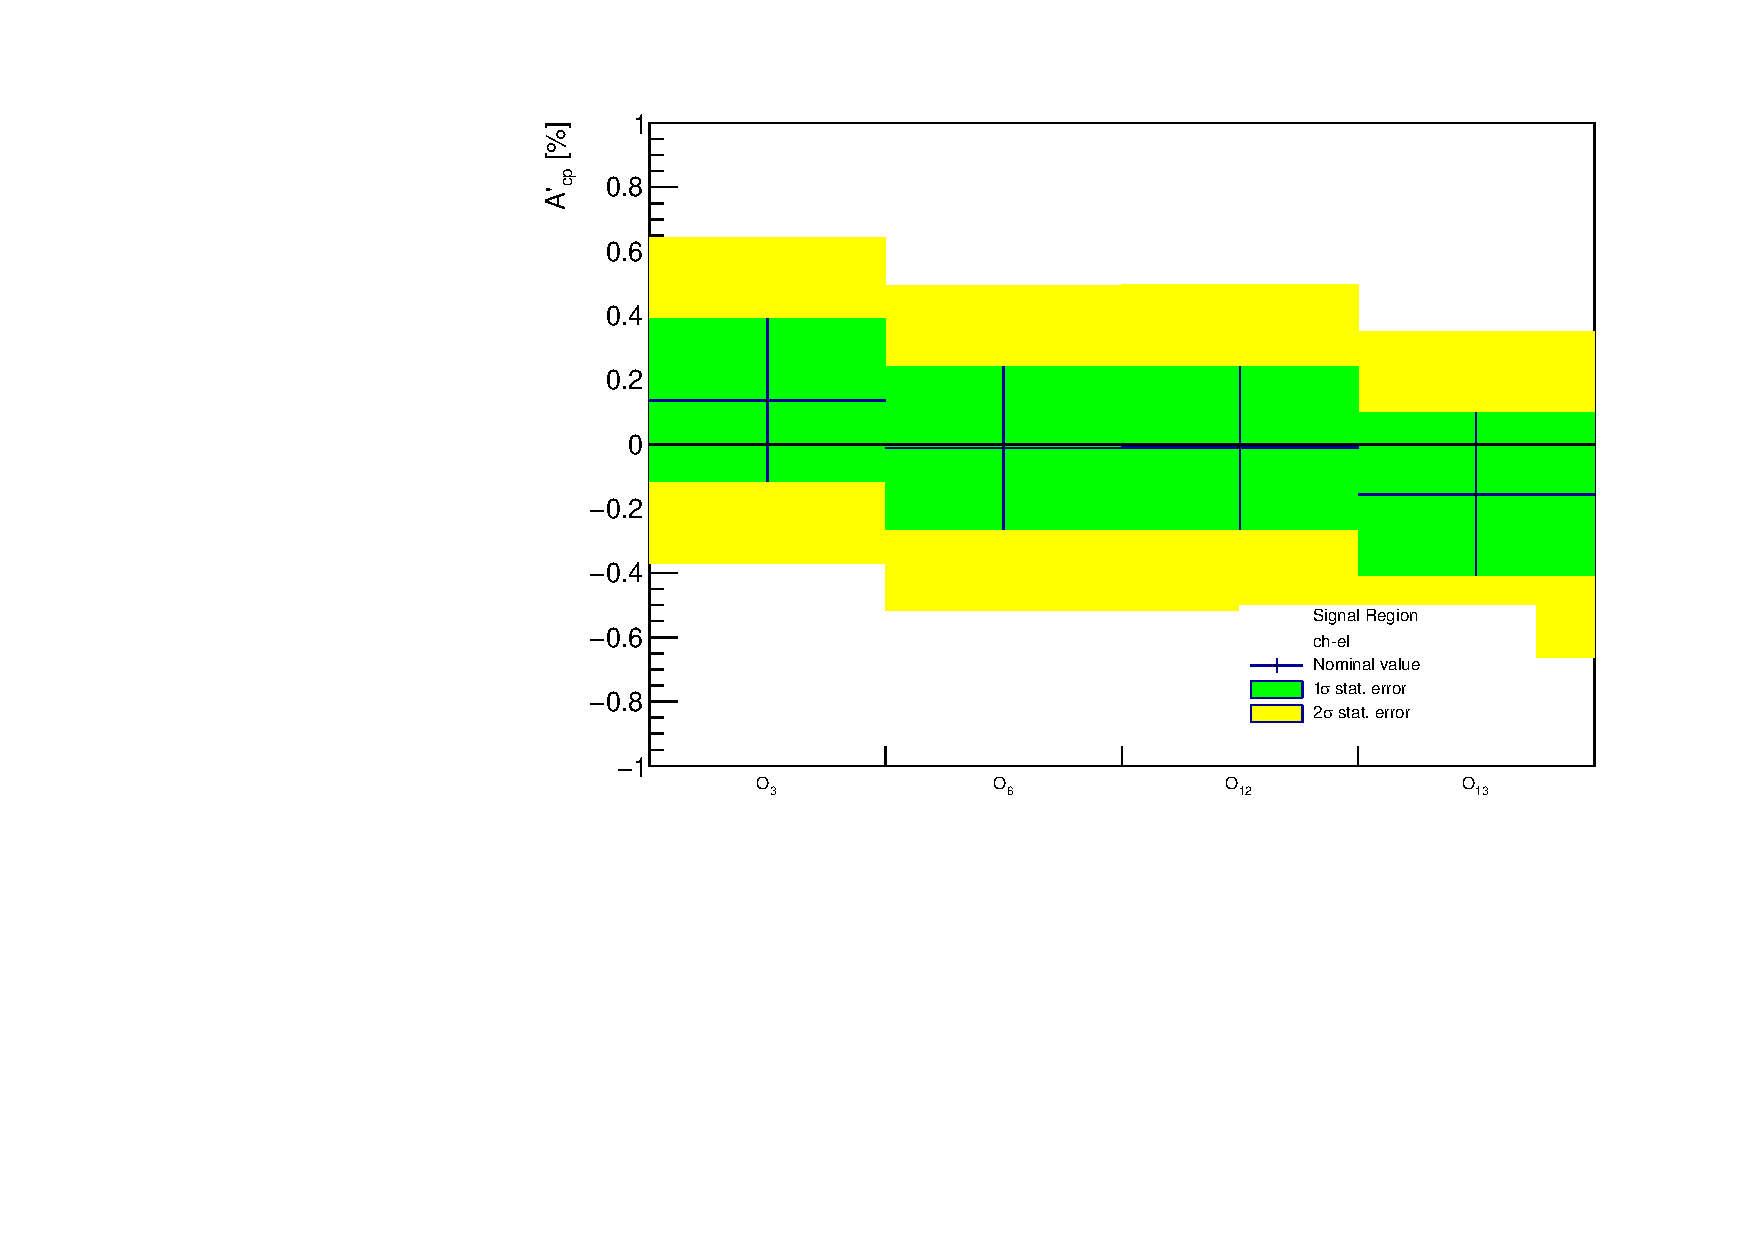
\includegraphics[width=0.45\textwidth]{Figures/Asym/check/Acp_a05_MLP_noMlbcut_DetBiasAcp_SRtt_200928_2219_el.pdf}}\\
		\caption{$A'_{cp}$ of simulated signal sample($t\bar{t}$) by MVA-B reconstruction strategy}
		\label{AsymBias:fig:a05_noMlbcut_sim_tt_A'cp}
		\end{figure}
		\FloatBarrier


		Futhermore, as previous mentioning, the $A'_{cp}$ of simulated background sample in SR is participated as a fine sample to check the detector and reconstruction bias. There are the checks whether they are has no asymmetry.

		\begin{figure}[H]
			\centering
				\subfigure[Muon channel]{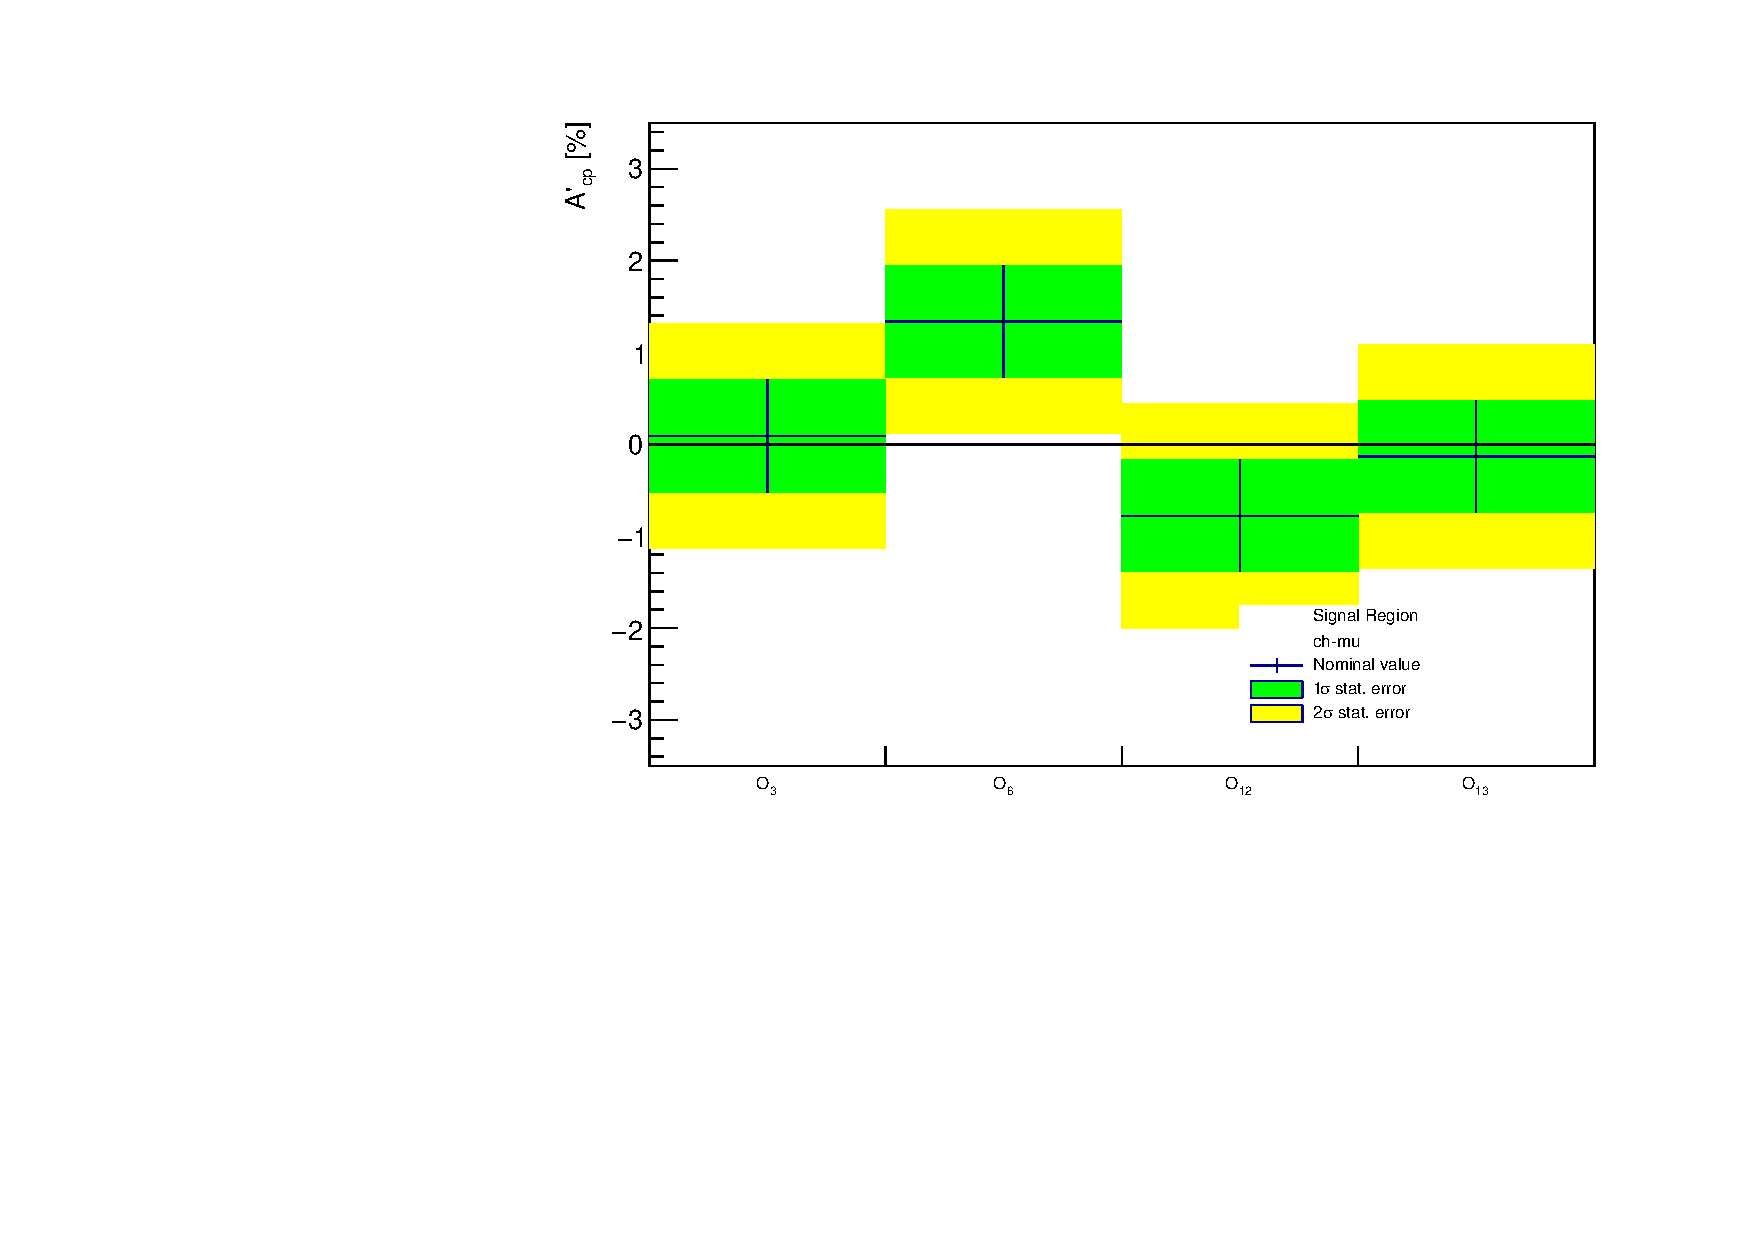
\includegraphics[width=0.45\textwidth]{Figures/Asym/check/Acp_chi2_Mlbcut_DetBiasAcp_SRbkg_200928_2207_mu.pdf}}
				\subfigure[Electron channel]{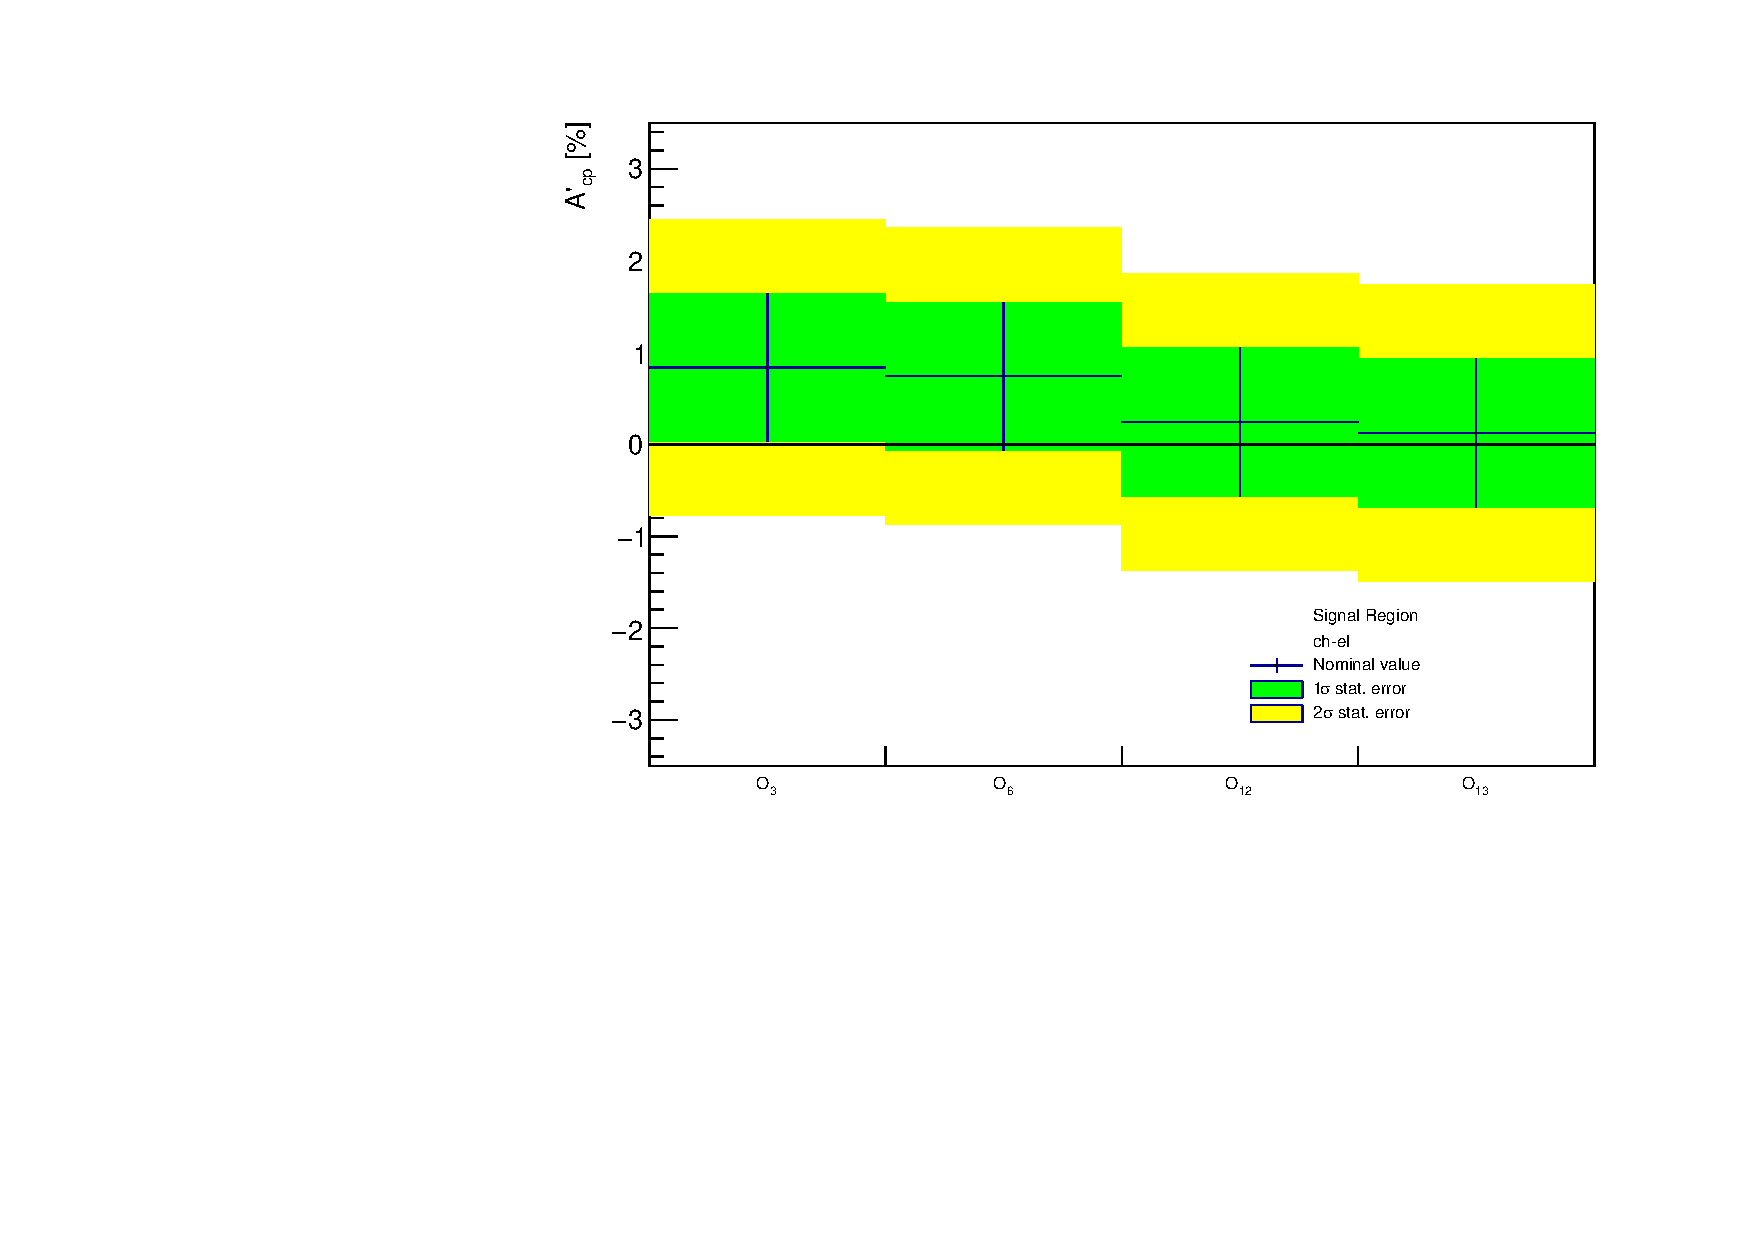
\includegraphics[width=0.45\textwidth]{Figures/Asym/check/Acp_chi2_Mlbcut_DetBiasAcp_SRbkg_200928_2207_el.pdf}}\\
		\caption{$A'_{cp}$ of simulated background sample by $\chi^2_{min}$ reconstruction strategy}
		\label{AsymBias:fig:chi2_sim_bkg_A'cp}
		\end{figure}
		\FloatBarrier

		\begin{figure}[H]
			\centering
				\subfigure[Muon channel]{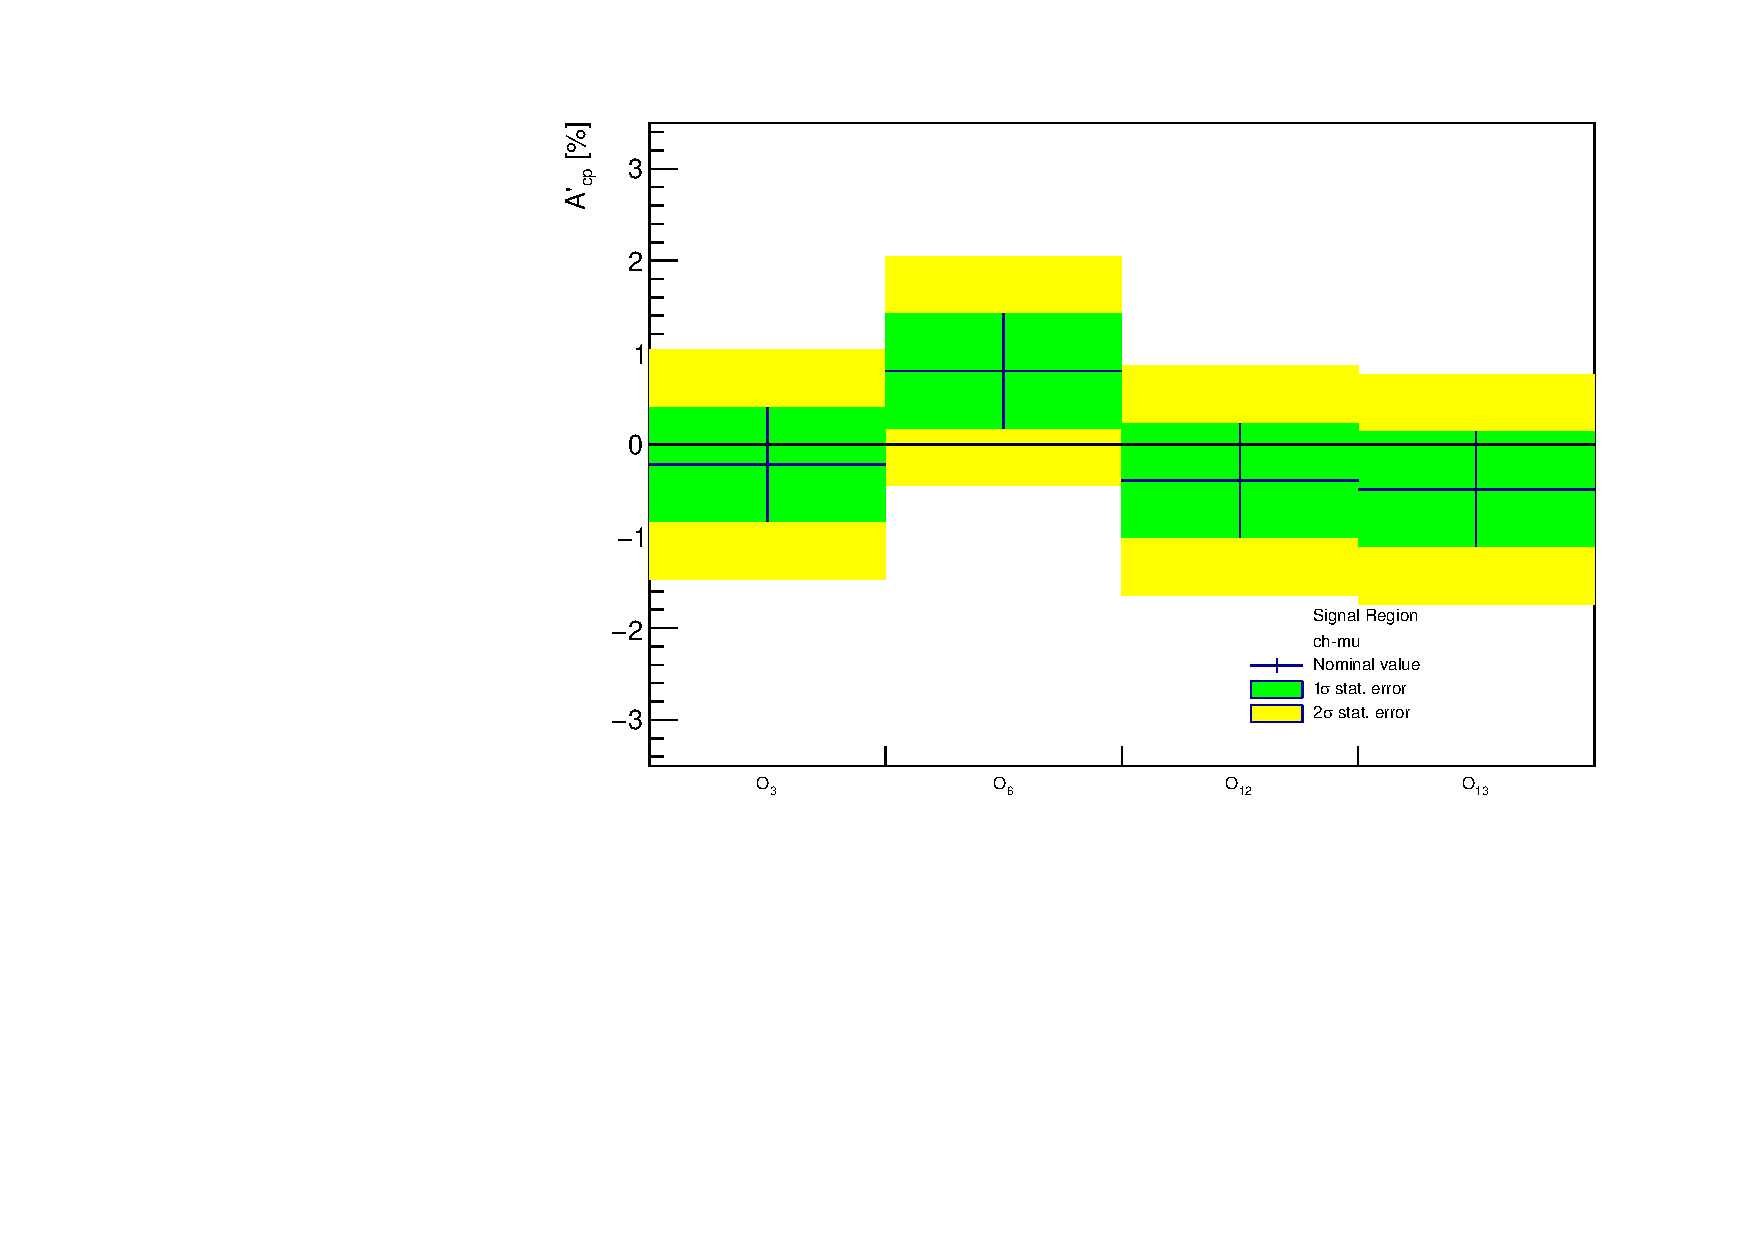
\includegraphics[width=0.45\textwidth]{Figures/Asym/check/Acp_a05_MLP_Mlbcut_DetBiasAcp_SRbkg_200928_2208_mu.pdf}}
				\subfigure[Electron channel]{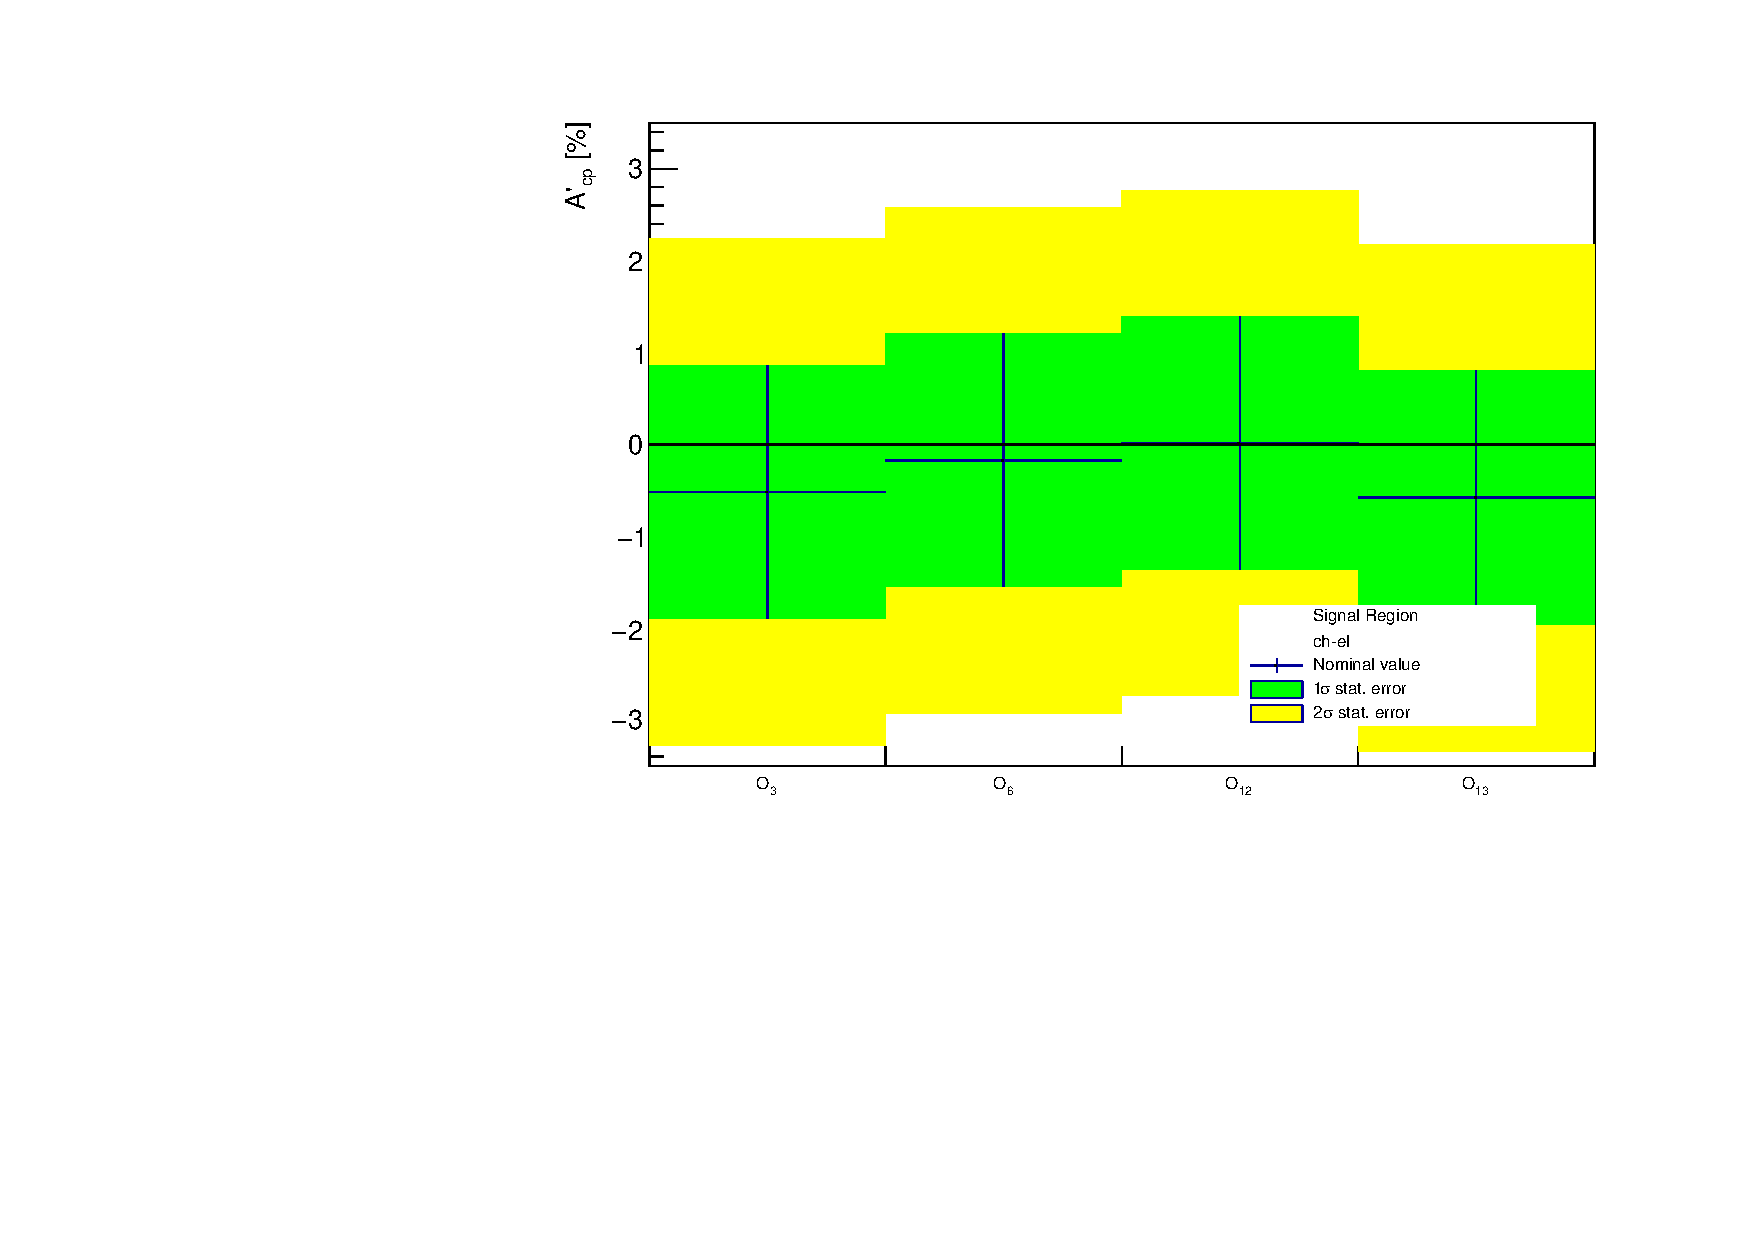
\includegraphics[width=0.45\textwidth]{Figures/Asym/check/Acp_a05_MLP_Mlbcut_DetBiasAcp_SRbkg_200928_2208_el.pdf}}\\
		\caption{$A'_{cp}$ of simulated background sample by MVA-A reconstruction strategy}
		\label{AsymBias:fig:a05_Mlbcut_sim_bkg_A'cp}
		\end{figure}
		\FloatBarrier

		\begin{figure}[H]
			\centering
				\subfigure[Muon channel]{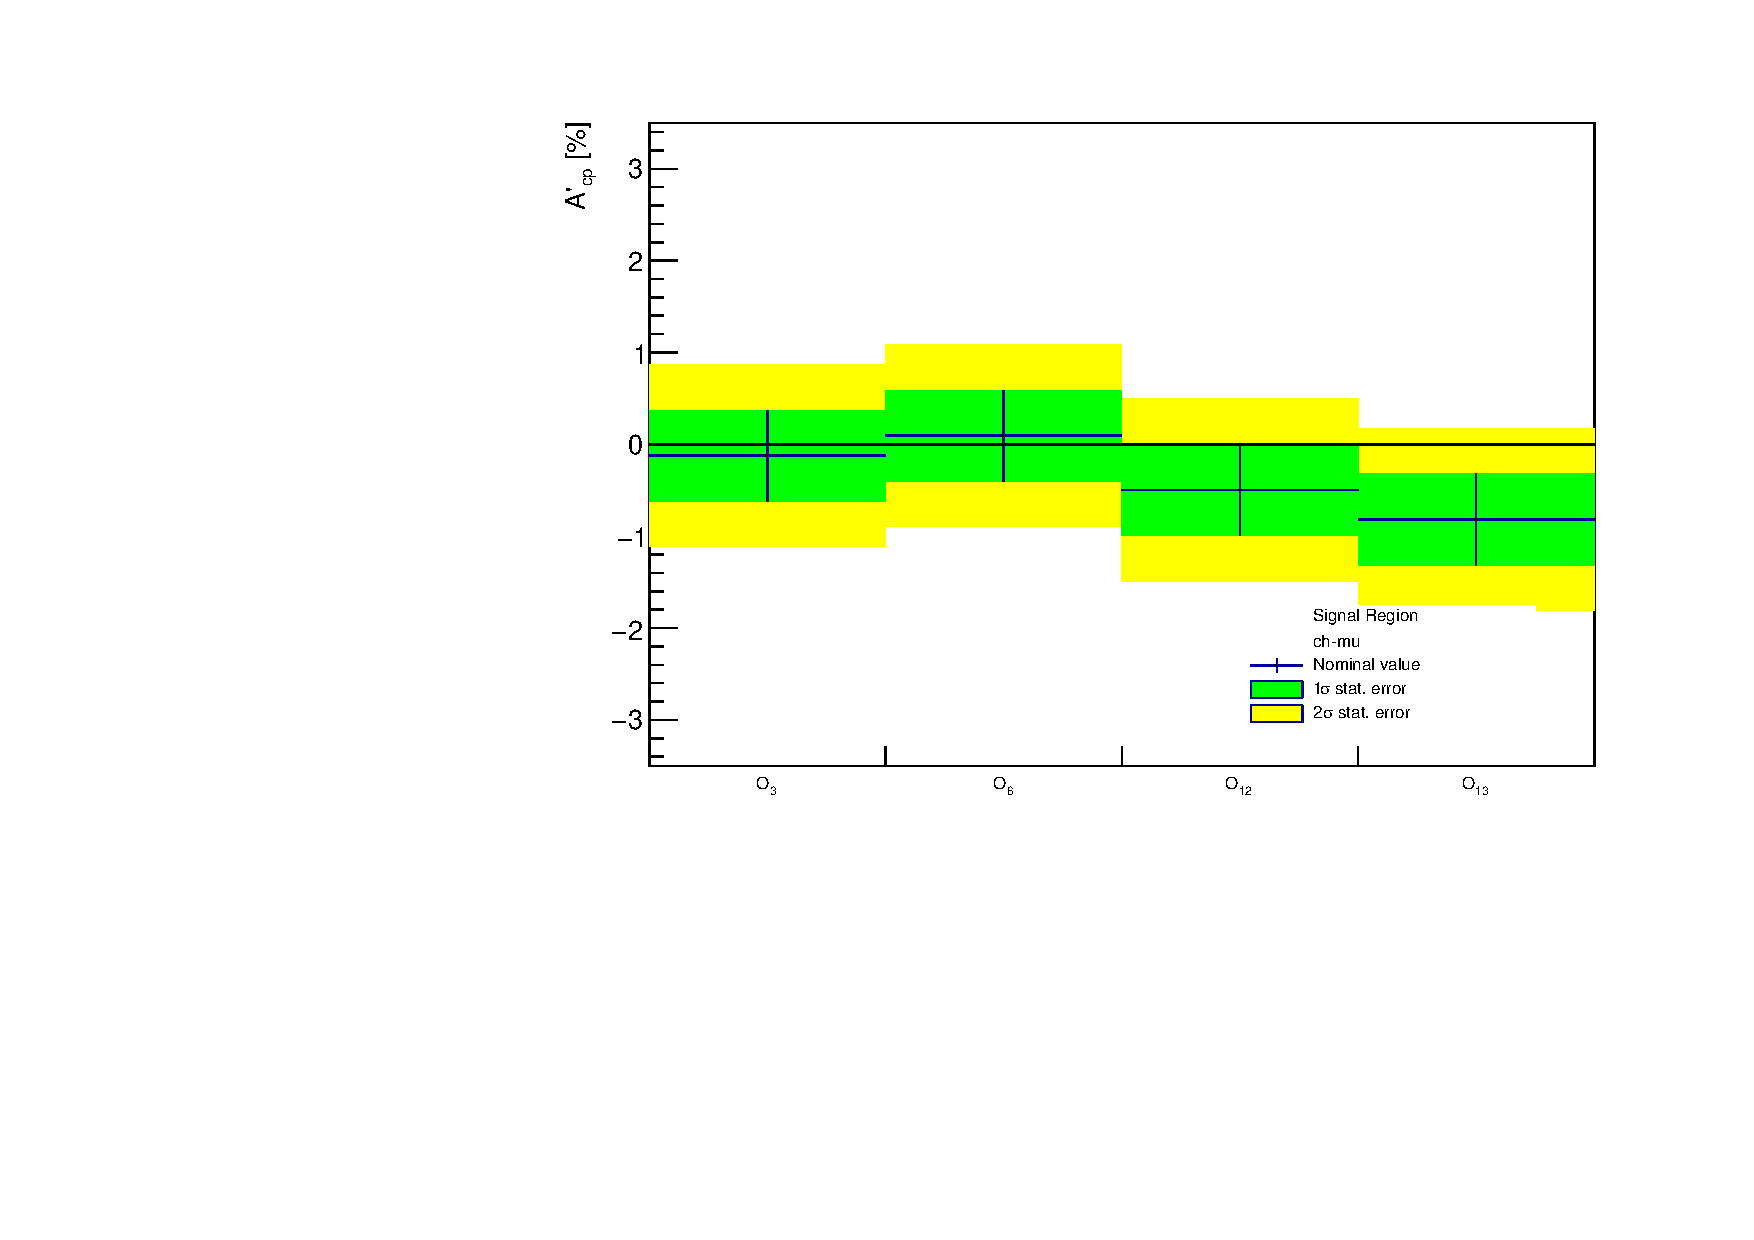
\includegraphics[width=0.45\textwidth]{Figures/Asym/check/Acp_a05_MLP_noMlbcut_DetBiasAcp_SRbkg_200928_2207_mu.pdf}}
				\subfigure[Electron channel]{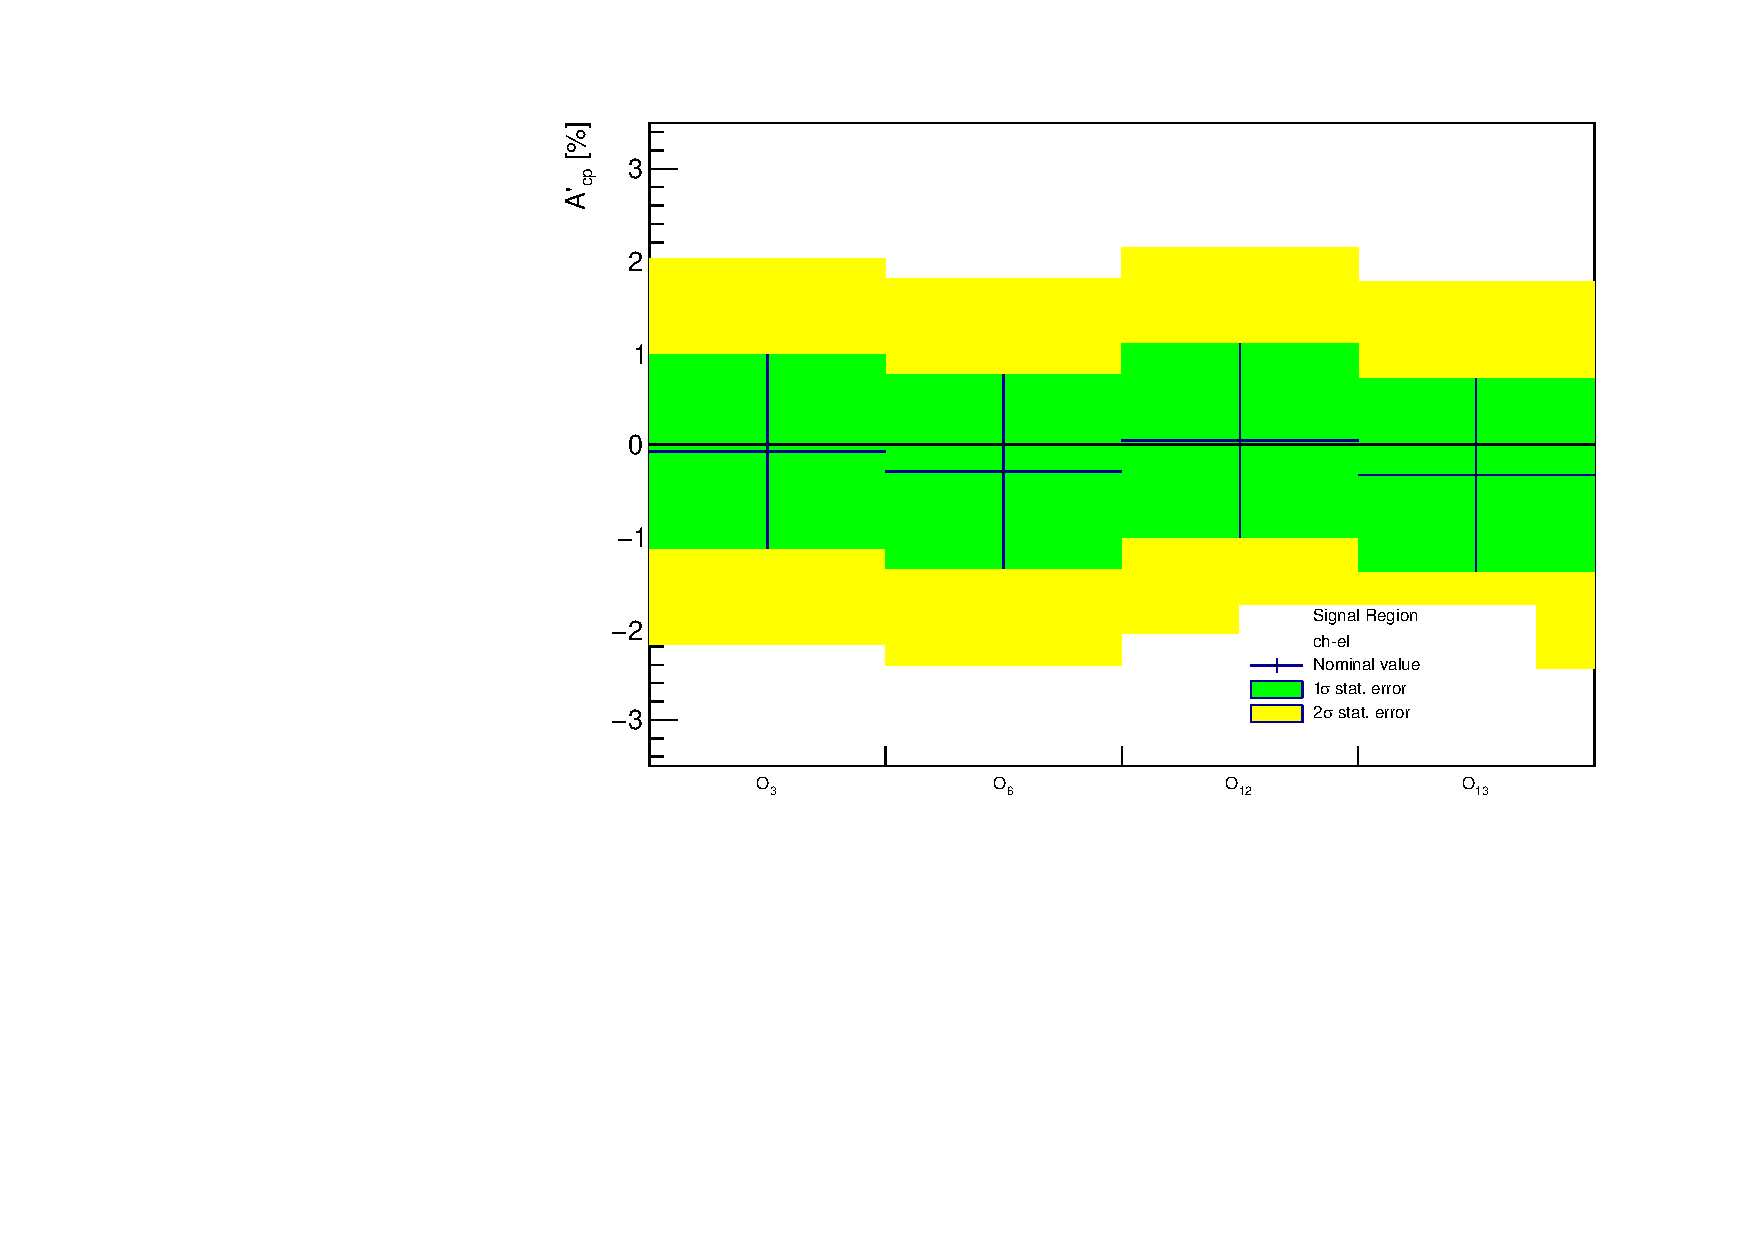
\includegraphics[width=0.45\textwidth]{Figures/Asym/check/Acp_a05_MLP_noMlbcut_DetBiasAcp_SRbkg_200928_2207_el.pdf}}\\
		\caption{$A'_{cp}$ of simulated background sample by MVA-B reconstruction strategy}
		\label{AsymBias:fig:a05_noMlbcut_sim_bkg_A'cp}
		\end{figure}
		\FloatBarrier

		The asymmetry of simulated signal and background sample in three reconstruction strategies are all in 2 statistical uncertainty and are regarded confirming without asymmetry.

	\subsection{Events mixing method}
	\label{ssec:evts_mixing}

		Using the real data of SR itself to make some fake-data sets can improve the measurerment of detector and reconstruction bias as systematic uncertainty. The method to make fake-data sets is called $\textbf{events mixing method}$. Events mixing method may discharge the effect of asymmetry of observables according to the structure of these triple-product observables.

		For the detail, the events mixing method is to pass both b-jet's and the leading light jet($j_1$)'s four momentum to the b-jet's and $j_1$'s four momentum of the next i-th event. Therefore, a chosen i gave a set of fake-data. For example, the 2nd set of fake-data is that, the first event's informations are passed to the third event, the second event's informations are passed to the fourth event, and the third event's informations are passed to the fifth event, etc. There is a reference graph of event mixing method(Fig.\ref{AsymBias:fig:event_mixing}).

		\begin{figure}[H]
		\centering{}
	    	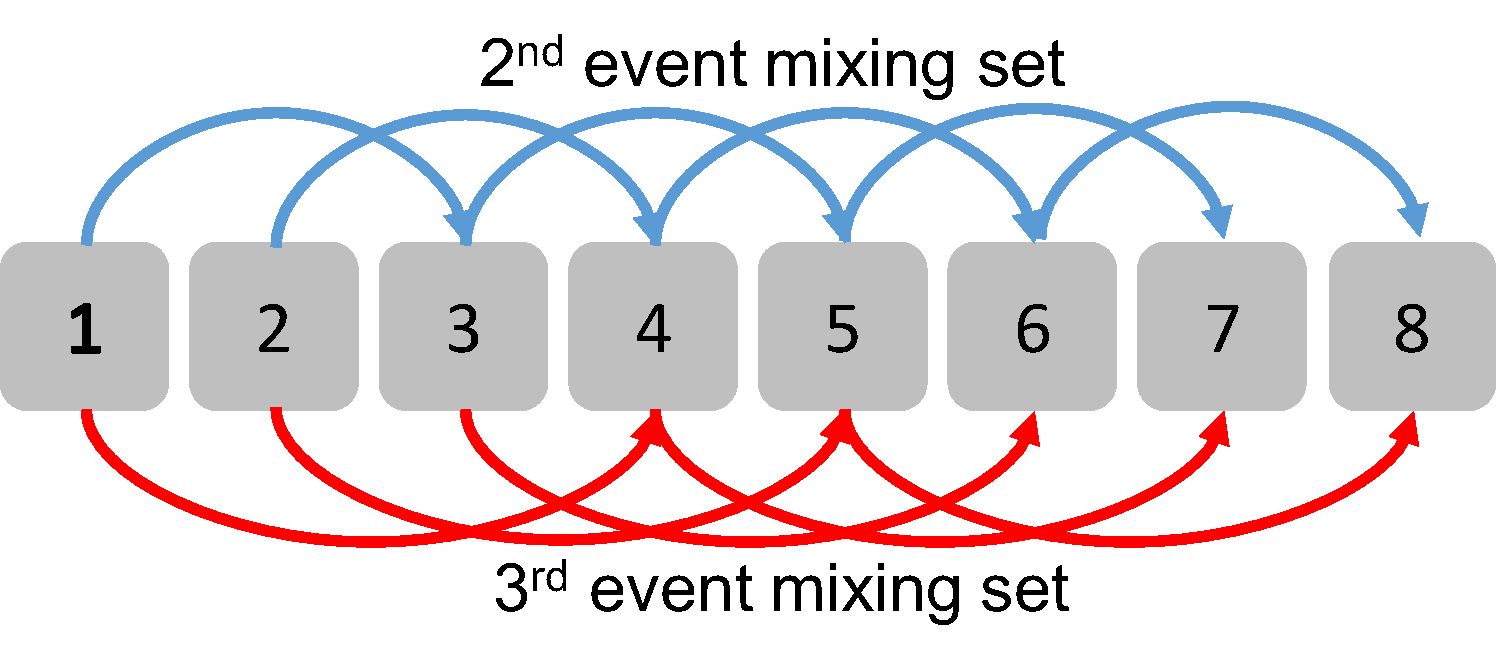
\includegraphics[width=0.65\textwidth]{Figures/Asym/event_mixing.pdf}\\
		\caption{Illustration graph of event mixing method}
		\label{AsymBias:fig:event_mixing}
		\end{figure}
		\FloatBarrier

		Before applying this method on real data to make fake data, it is needed to check whether the events mixing method really mix the information of particle kinematics and really cancel out the intrinsic asymmetry factor. To check the canceling out effect, there is an artificial generated $A'_{cp}$ sample prepared by duplicating random positive events with given probability. Then apply the event mixing result on this sample, the results are shown below(Fig.\ref{AsymBias:fig:washout_artificial}), and we can confirm that the method would really cancel out the $A'_{cp}$.

		\begin{figure}[H]
		\centering{}
	    	\subfigure[Muon channel]{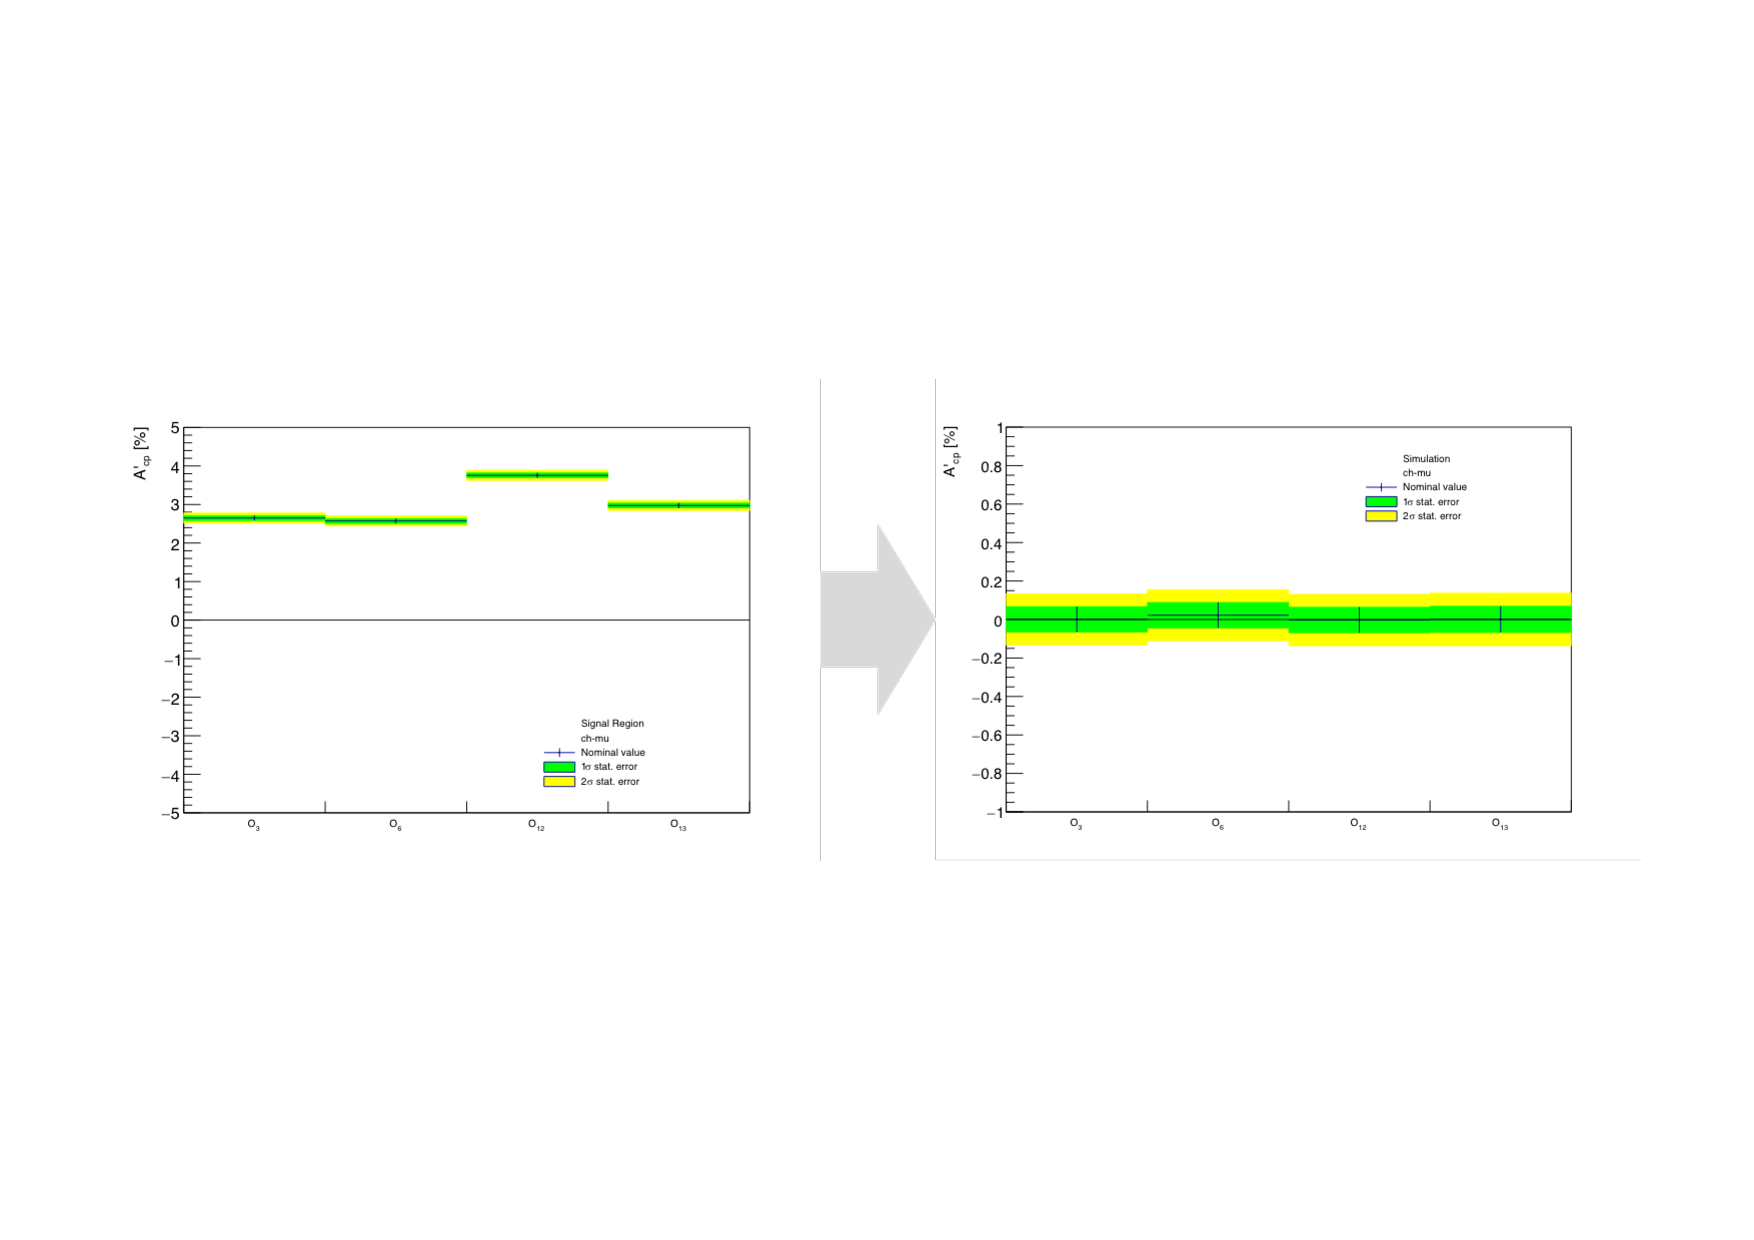
\includegraphics[width=0.85\textwidth]{Figures/Asym/artificial/a05_artificial_to_mix_mu.pdf}}\\
		\end{figure}
		\FloatBarrier
		\begin{figure}[H]
		\centering{}
	    	\subfigure[Electron channel]{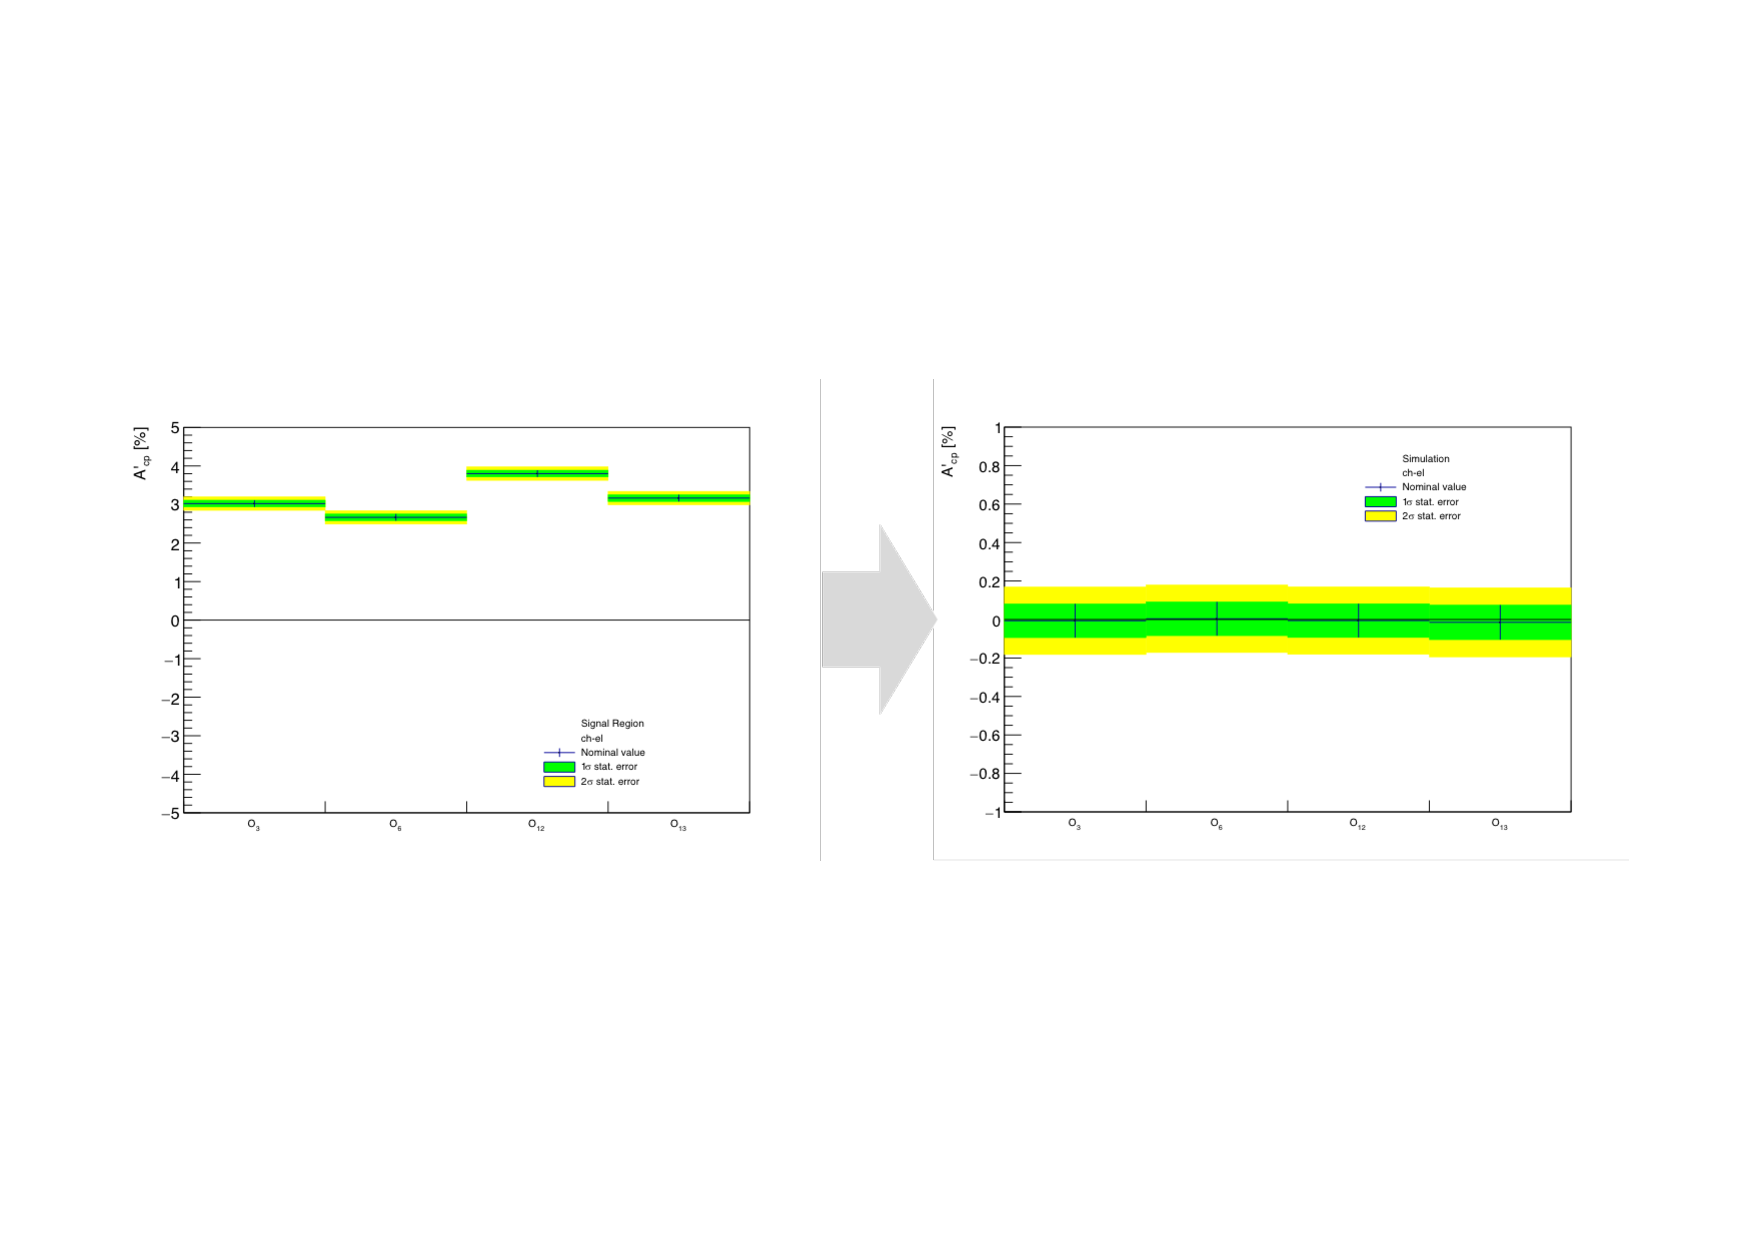
\includegraphics[width=0.85\textwidth]{Figures/Asym/artificial/a05_artificial_to_mix_el.pdf}}\\
		\caption{}
		\label{AsymBias:fig:washout_artificial}
		\end{figure}
		\FloatBarrier

		And then to get the reconstruction and detector bias, we generate 1000 sets of fake-data samples.Then, we measure their $A'_{cp}$, and average the 1000 results mean values and standard deviations. The derived standard deviations of 4 observables are considered as the detector and reconstruction bias also the major systematic uncertainty of the 4 observables' final results. There are the plots of reconstruction and detector bias with event mixing method under three reconstruction strategies($\chi^2_{min}$, MVA-A, MVA-B):

		\begin{figure}[H]
			\centering
				\subfigure[Muon channel]{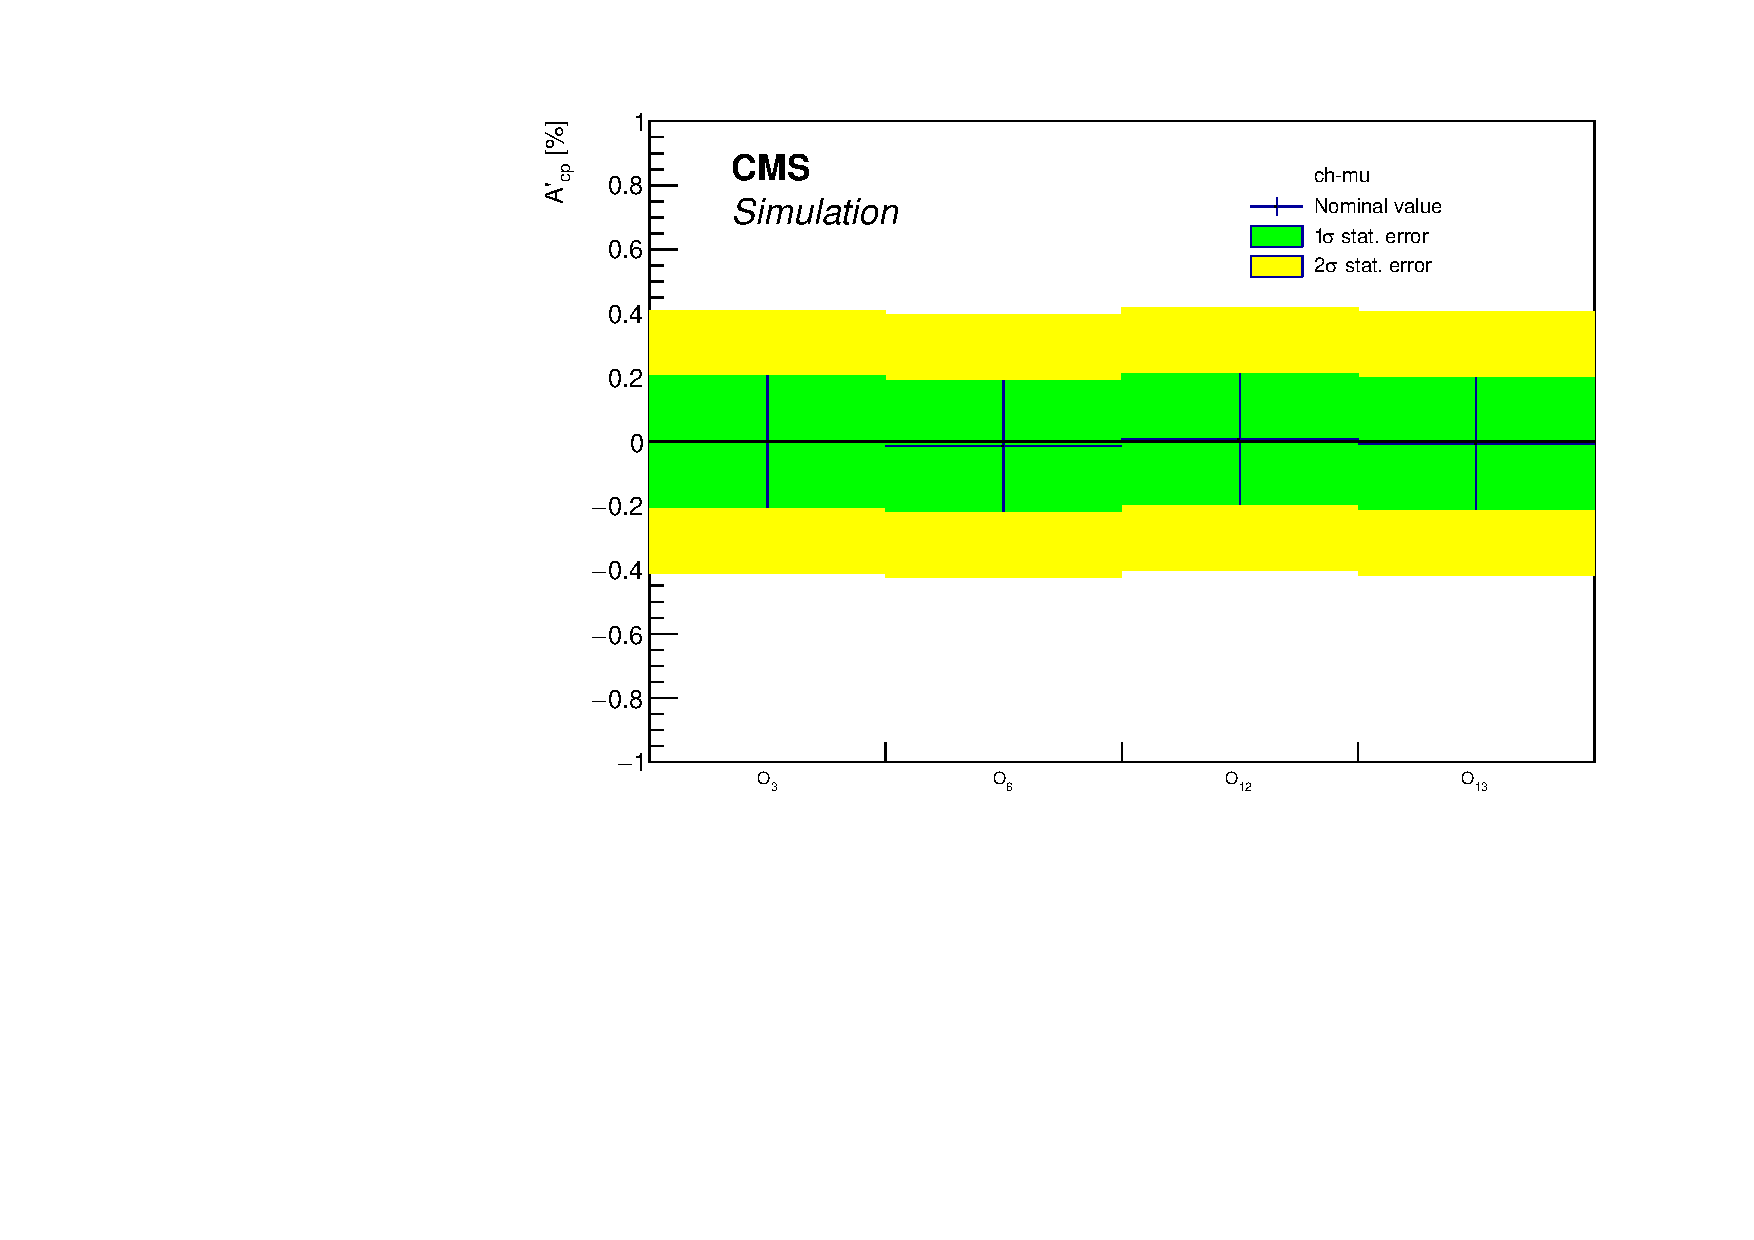
\includegraphics[width=0.45\textwidth]{Figures/Asym/DetBias/Acp_chi2_fakeData_ChangeInfo_mu.pdf}}
				\subfigure[Electron channel]{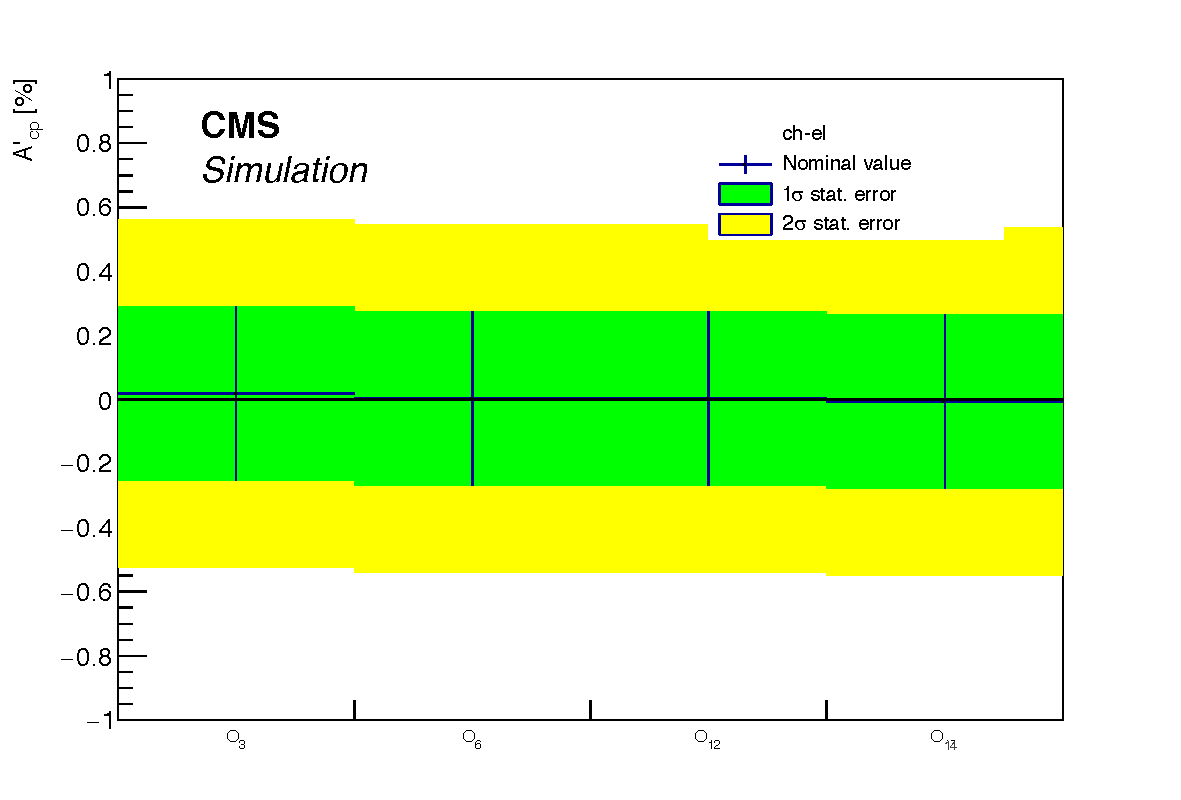
\includegraphics[width=0.45\textwidth]{Figures/Asym/DetBias/Acp_chi2_fakeData_ChangeInfo_el.pdf}}\\
		\caption{average $A'_{cp}$ of 1000 sets fake-data by $\chi^2_{min}$ reconstruction strategy}
		\label{AsymBias:fig:chi2_DetBias}
		\end{figure}
		\FloatBarrier

		\begin{figure}[H]
			\centering
				\subfigure[Muon channel]{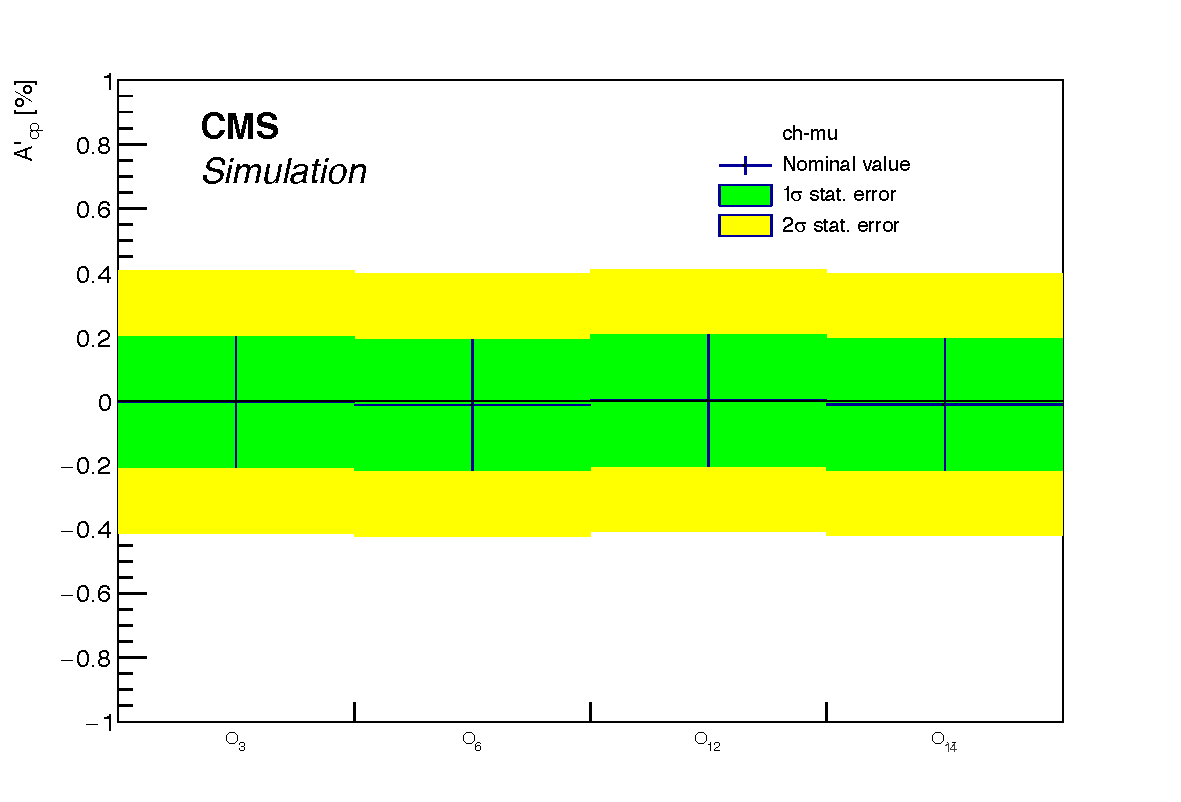
\includegraphics[width=0.45\textwidth]{Figures/Asym/DetBias/Acp_a05_all_MLP_fakeData_ChangeInfo_mu.pdf}}
				\subfigure[Electron channel]{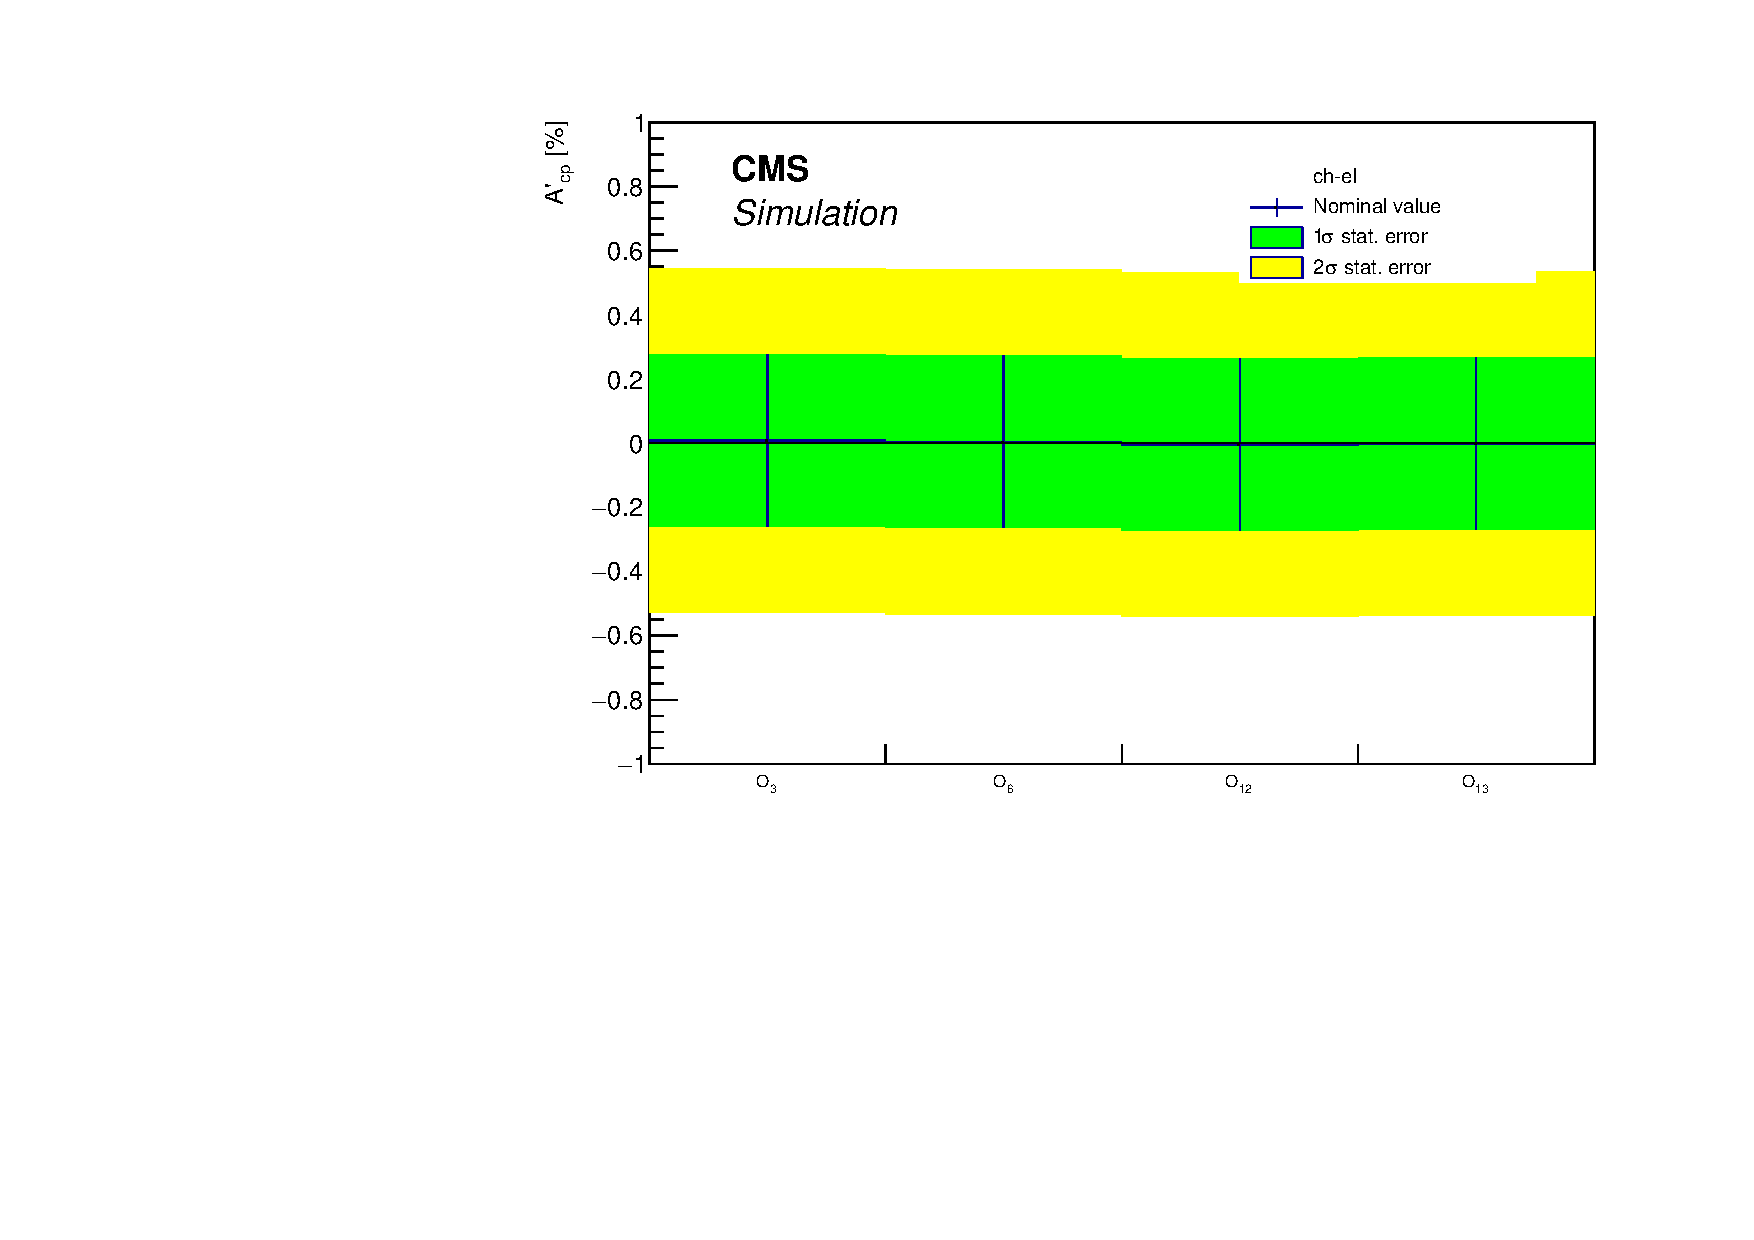
\includegraphics[width=0.45\textwidth]{Figures/Asym/DetBias/Acp_a05_all_MLP_fakeData_ChangeInfo_el.pdf}}\\
		\caption{average $A'_{cp}$ of 1000 sets fake-data by MVA-A reconstruction strategy}
		\label{AsymBias:fig:a05_Mlbcut_DetBias}
		\end{figure}
		\FloatBarrier

		\begin{figure}[H]
			\centering
				\subfigure[Muon channel]{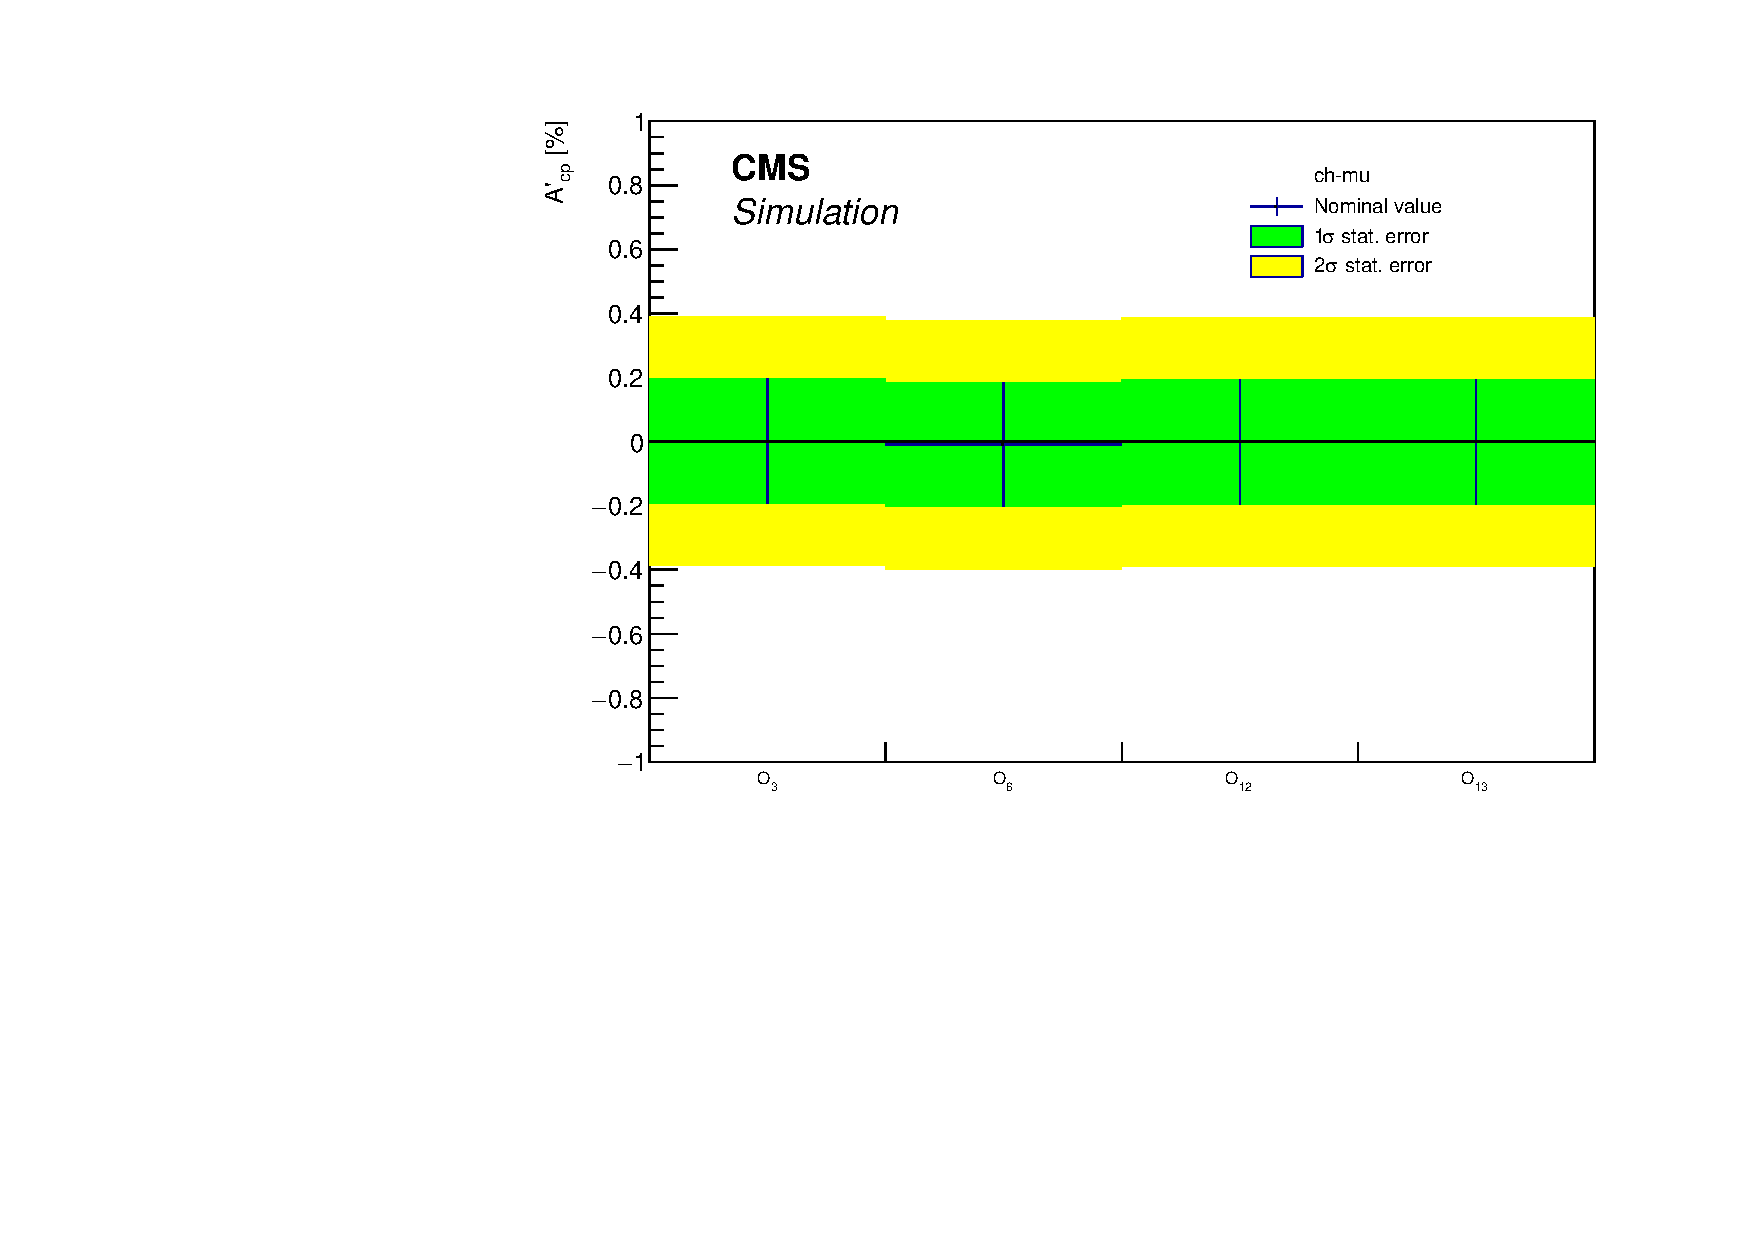
\includegraphics[width=0.45\textwidth]{Figures/Asym/DetBias/Acp_a05_all_MLP_MlbNo_fakeData_ChangeInfo_mu.pdf}}
				\subfigure[Electron channel]{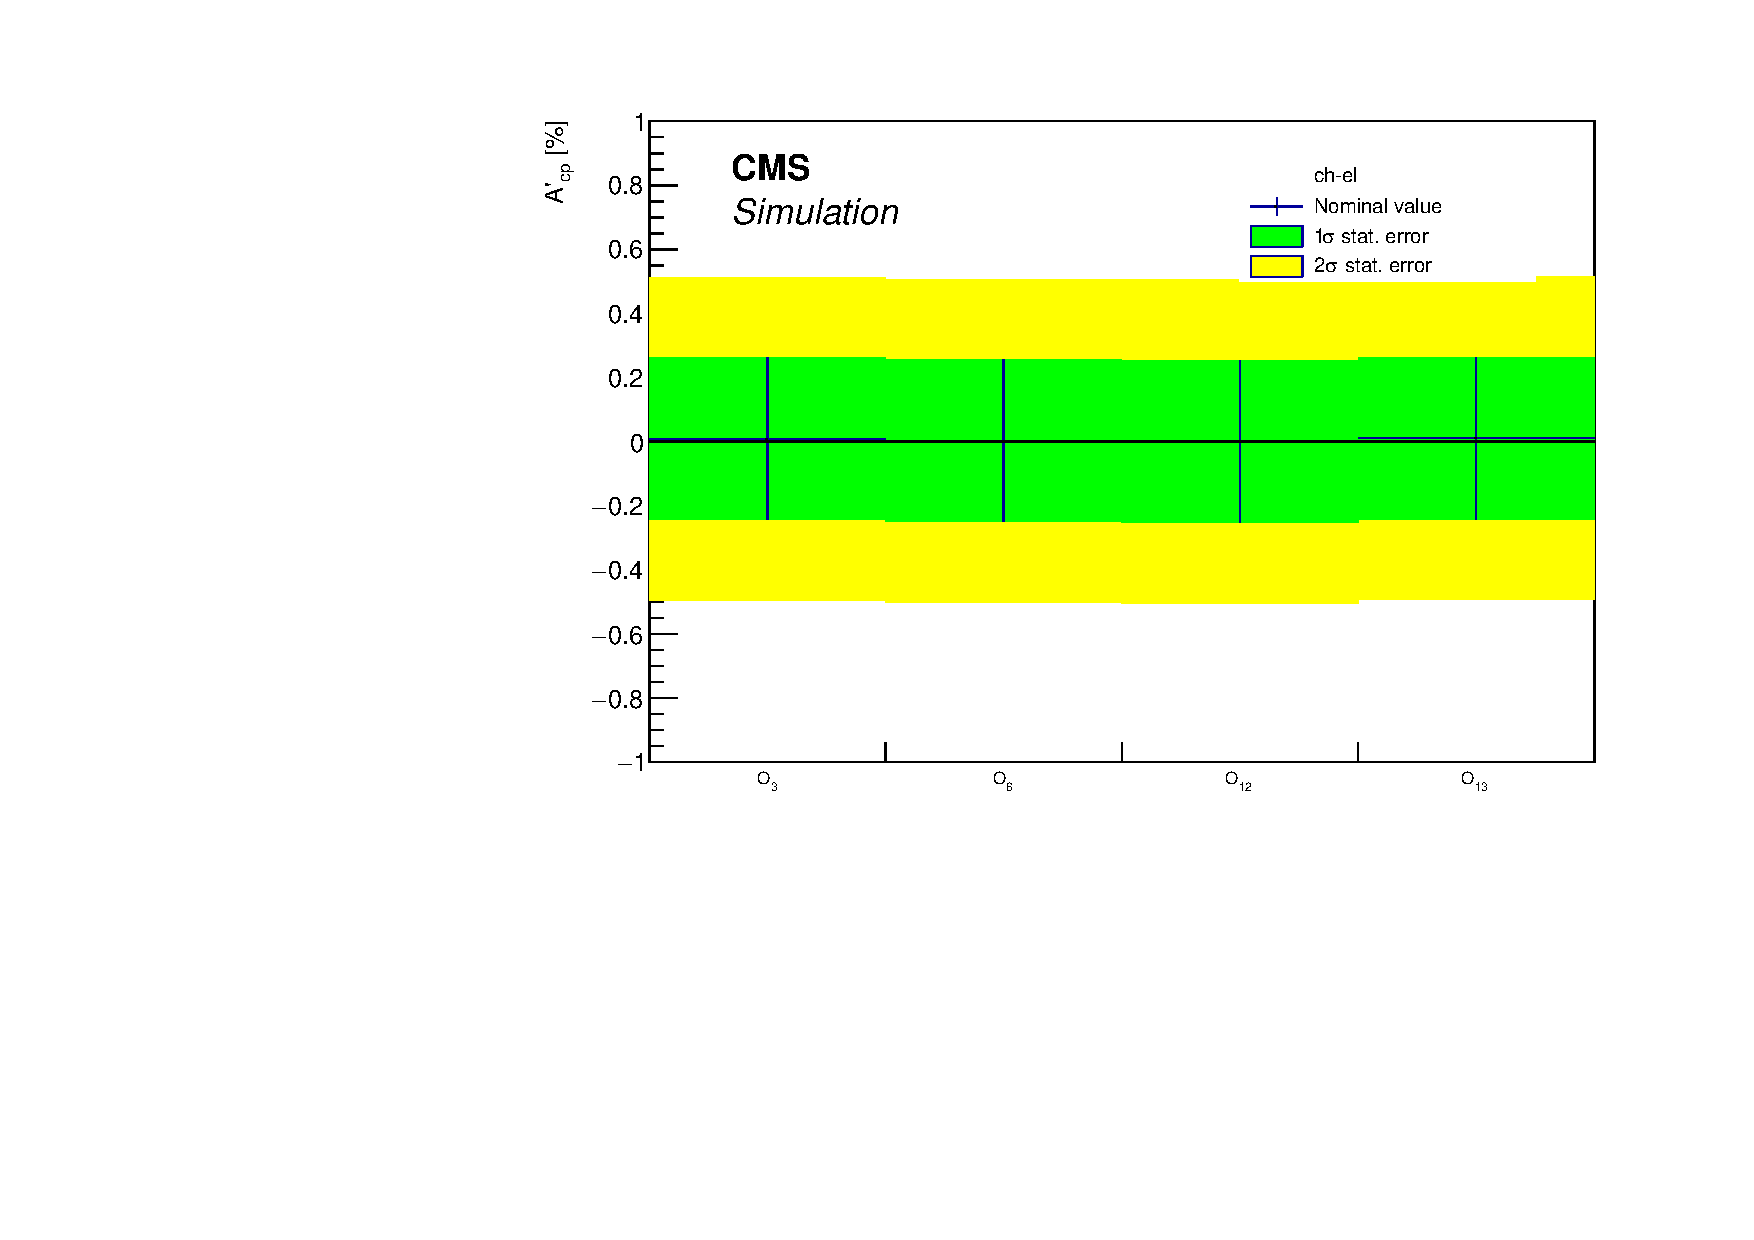
\includegraphics[width=0.45\textwidth]{Figures/Asym/DetBias/Acp_a05_all_MLP_MlbNo_fakeData_ChangeInfo_el.pdf}}\\
		\caption{average $A'_{cp}$ of 1000 sets fake-data by MVA-B reconstruction strategy}
		\label{AsymBias:fig:a05_noMlbcut_DetBias}
		\end{figure}
		\FloatBarrier


		\begin{center}
		\begin{longtable}[H]{ c c c c c c }
		\caption{Reconstruction and detector bias of $\chi^2_{min}$ strategy}\\
		\hline
		[\%] & $O_{3}$ & $O_{6}$ & $O_{12}$ & $O_{14}$ \\ 
		\hline{}
		Muon channel & $\pm0.205$ & $\pm0.205$ & $\pm0.205$ & $\pm0.205$ \\
		Electron channel & $\pm0.271$ & $\pm0.271$ & $\pm0.271$ & $\pm0.271$ \\
		\hline
		\label{AsymBias:tb:chi2_DetBias}
		\end{longtable}
		\end{center}

		\begin{center}
		\begin{longtable}[H]{ c c c c c c }
		\caption{Reconstruction and detector bias of MVA-A strategy}\\
		\hline
		[\%] & $O_{3}$ & $O_{6}$ & $O_{12}$ & $O_{14}$ \\ 
		\hline{}
		Muon channel & $\pm0.204$ & $\pm0.204$ & $\pm0.204$ & $\pm0.204$ \\
		Electron channel & $\pm0.268$ & $\pm0.268$ & $\pm0.268$ & $\pm0.268$ \\
		\hline
		\label{AsymBias:tb:a05_Mlbcut_DetBias}
		\end{longtable}
		\end{center}

		\begin{center}
		\begin{longtable}[H]{ c c c c c c }
		\caption{Reconstruction and detector bias of MVA-B strategy}\\
		\hline
		[\%] & $O_{3}$ & $O_{6}$ & $O_{12}$ & $O_{14}$ \\ 
		\hline{}
		Muon channel & $\pm0.194$ & $\pm0.194$ & $\pm0.194$ & $\pm0.194$ \\
		Electron channel & $\pm0.252$ & $\pm0.252$ & $\pm0.252$ & $\pm0.252$ \\
		\hline
		\label{AsymBias:tb:a05_noMlbcut_DetBias}
		\end{longtable}
		\end{center}

\FloatBarrier
